\documentclass[pdftex,letterpaper,12pt]{report}
\usepackage{thesis}
\usepackage{amsmath}
\usepackage{amssymb}
\usepackage{amsthm}
\usepackage{mathtools}
\usepackage{bm}
\usepackage{gensymb}
\usepackage{wasysym}
\usepackage{mathtools}
\usepackage{physics}
\usepackage{empheq}
\usepackage{cases}
\usepackage{rotating}
\usepackage{subfig}
\usepackage{caption}
\usepackage{multirow}
\captionsetup{labelfont=bf} 
\captionsetup[subfloat]{position=top,singlelinecheck=off,justification=raggedright,font=bf,labelfont=large,labelformat=simple,captionskip=-2mm}
\usepackage{float}
\usepackage{enumitem} 
\usepackage[toc,page]{appendix}






\begin{document}
	
\pagenumbering{roman}

\thesistitle
{Next-Generation Polarized $^3$He Targets for Electron Scattering Experiments}                                                % title
{Yunxiao Wang}                                               % author
{Anqing, Anhui, China}                               % hometown
{B.S. in Physics University of Science and Technology of China May 2009} % previous degree(s)
{Doctor of Philosophy}                                 % degree to be defensed
{Department of Physics}                                % department/school
{Dec, 2016}  

%\pagenumbering{roman}

%\thesistitle
%	{Next-Generation Polarized $^3$He Targets for Electron Scattering Experiments}
%	{Yunxiao Wang}
%	{Doctor of Philosophy}
%	{Department of Physics}
%	{November 2016}

%\thesistitle
%	{My Thesis Title}                                                % title
%	{Yunxiao Wang}                                               % author
%	{Anqing, Anhui, China}                               % hometown
%	{B.S. in Physics University of Science and Technology of China May 2009} % previous degree(s)
%	{Doctor of Philosophy}                                 % degree to be defensed
%	{Department of Physics}                                % department/school
%	{Nov, 2016}                                            % date

\addcontentsline{toc}{chapter}{Abstract}
\begin{center}
	\textbf{\large Abstract}
\end{center}

Historically, $^3$He targets for electron scattering experiments have been polarized through spin-exchange optical pumping (SEOP). Polarized laser light passes its circular polarization to alkali metal vapor, which then transfers its polarization to $^3$He through spin-exchange collisions. 

This thesis discusses the basics of SEOP and the polarimetry techniques used in our lab. Narrowband laser and alkali-hybrid SEOP have improved the performance of targets significantly. In alkali-hybrid SEOP, potassium is used together with rubidium for transferring polarization to $^3$He nuclei. We discussed the data collected over many pure-rubidium targets and alkali-hybrid targets. In the course of analyzing the data, we also studied the ``X factor" which limits the highest achievable polarization of $^3$He.

Because the experiments planned for the 12GeV era in Jefferson National Laboratory (JLAB) will use much higher electron beam current, we are exploring the possibility of using metal (instead of glass) as the entry points (commonly referred to as ``end windows") for future targets. We established the metal composition and developed the techniques to incorporate metal to targets without introducing significant spin-relaxation rates. We have successfully demonstrated that future targets can be constructed with metal end windows and are very close to making such targets.
\addcontentsline{toc}{chapter}{Acknowledgements}
\begin{center}
\textbf{\large Acknowledgements}
\end{center}

First and foremost, I'd like to give my thanks to my advisor, Gordon Cates, for supporting me in the past five years in the group. Not only because I have learned a lot about physics from you, but also for your incredible enthusiasm that kept motivating me to push towards earning my degree. I am honored to have worked with you.

I'd like to thank Peter Dolph and Yuan Zheng, who have taught me the basics of spin-exchange optical pumping and $^3$He and alkali polarimetry. Even though the time we spent working together was not long, it laid the very foundation for my work in the following years.

I would like to thank Dr. W. Al Tobias and Dr. Vladimir Nelyubin as well. Al has helped us fill almost every cell we have studied and also taught me the right way to do experiments and the importance of documentation. Vladimir always made sure our experiments could go as smoothly as possible with his laser expertise. We would not have been able to do it without the help from Al and Vladimir.

I also would like to thank all the other graduate students in the group. Maduka Kaluarachchi and Dan Matyas, the two of you made the hours in lab such a joy. I will always miss our talks and of course, the "Young Chicken" we shared at Taste of China. Graduate school was not an easy time for me, I could not have done it without the help from you guys. Sumudu Katugampola and Dave Keder, the two of you are already doing great work, I have no doubt that you will have tremendous amount of success in the future. I look forward to seeing what our lab will be able to achieve because of you.

I'd like to thank the members of my committee: Nilanga Liyanage, Don Crabb, Wilson Miller, for helping me complete the final step towards my degree. I also owe my thanks to my parents and all my friends who have supported me through all these years. It means a lot to me knowing that no matter what comes next, I will always have your support.

Last but not least, I would like to thank my girlfriend. Shuangshuang, every bit of success I was able to achieve since I met you was at least partly because of your love and support. You gave me something to hold on to so I could pull myself through a tough time. I would not have been able to move on to the next chapter of my life the same way I did without you.



%\vspace{1cm}

%\emph{``Intellectual and practical assistance, advice, encouragement and
%sources of monetary support should be acknowledged. It is appropriate to
%acknowledge the prior publication of any material included in the thesis
%either in this section or in the introductory chapter of the thesis.''}

%\hfill --- MUN School of Graduate Studies

\include{contents}
\include{tables}
\include{figures}

\pagenumbering{arabic}
\chapter{Introduction}
\label{chap:chap1}

Nuclear-polarized noble gases have been proven to be very useful in various applications, such as polarized targets for electron scattering experiments~\cite{PhysRevLett.71.959}, magnetic resonance imaging~\cite{MRI} and neutron scattering experiments~\cite{Neutron}. Polarized $^3$He has been particularly useful for studying spin-dependent interactions involving neutrons because, to first-order approximation, a $^{3}$He nucleus has a pair of protons with paired spins and a single neutron that carries most of the nuclear spin. Free neutrons are not used as targets because they decay with a lifetime of about 14 minutes, 42 seconds. 

\section{Motivation and Approved JLab Experiments}

The neutron electromagnetic form factors, $G_E^n$ and $G_M^n$ play essential roles for understanding nucleon structure. At non-relativistic energies, they are the Fourier transforms of the electric charge and magnetic moment distributions. Even at relativistic energies, the elastic form factors provide unique information on the transverse structure of the nucleon~\cite{PhysRevLett.99.112001, PhysRevLett.100.032004}. Double-polarization experiments on the proton showed that the ratio of the proton's electric and magnetic elastic form factors, $G_E^p/G_M^p$, declines nearly linearly as the four momentum transfer squared, $Q^2$, increases, in sharp contrast to expectations~\cite{PhysRevLett.84.1398}. These measurements caused a resurgence of interest in nucleon structure, and shed light on the importance of quark orbital angular momentum. More recent double-polarization experiments measured the neutron electric form factor $G_E^n$ up to a $Q^2$ of $\rm 3.4\,GeV^2$ (E02-013)~\cite{Phys.Rev.Lett.105.262302}, and showed behavior that was generally consistent with models that described well the earlier proton results. The neutron results, when combined with the proton results, also made it possible to extract the form factors for the individual up- and down-quark flavors~\cite{PhysRevLett.106.252003}. Significantly different $Q^2$ dependence was seen for the up- and down-quarks, a difference that some theorists have interpreted as evidence for the importance of diquark correlations.  

The multiple surprises that have emerged from the study of nucleon elastic form factors at Jefferson Laboratory (JLab) have underscored the value of performing such studies at high values of $Q^2$. For the neutron, predictions for the behavior of the ratio of the electric and magnetic elastic form factors, $G_E^n/G_M^n$, vary significantly from one model or calculation to another. A particularly compelling example, based on the Dyson-Schwinger Equation (DSE) formalism, predicts a dramatic turnover and zero crossing in the vicinity of $Q^2 = \rm 10\,GeV^2$~\cite{Cloet}. The verification of this prediction would have profound impact on our understanding of nucleon structure. An important part of the future program at JLab to explore the high-$Q^2$ behavior of the elastic nucleon form factors is the Super Bigbite Spectrometer (SBS) program. The SBS experiment to measure $G_E^n/G_M^n$ up to $Q^2 = \rm 10\,GeV^2$, E12-09-016, is a major motivating factor for the work described in this thesis. The count rate associated with the elastic form factors drops off very quickly with increasing $Q^2$. This in turn puts pressure on all aspects of the experiment to achieve adequate statistics, including running the polarized $^3$He target at high luminosity.  

Another important issue in understanding nucleon structure is the spin structure associated with the quarks. Polarized deep inelastic scattering provides a window into the spin carried by the quarks, and a particularly useful observable is the spin asymmetry $A_1^n$, that describes the spin dependence of the virtual photo absorption cross section. It is particularly useful to measure $A_1^n$ at high values of Bjorken $x$, where several predictions exist. Both constituent quark models and perturbative QCD predict that $A_1^n \rightarrow 1$ as $x_{\rm Bj} \rightarrow 1$, but it is also the case that count rates drop quickly toward high values of  $x_{\rm Bj}$. Two experiments are currently approved at JLab that will measure $A_1^n$ up values of  $x_{\rm Bj}$ in excess of 0.7; they are E12-06-122 in Hall A, and E12-06-110 in Hall C. Both of these experiments will require a polarized $^3$He target capable of running at high luminosity and thus depend critically on the work describe here.  

\section{Overview of Recent Target Development}

An early use of polarized $^3$He targets in electron scattering experiments was at the Stanford Linear Accelerator Center (SLAC) in the year of 1992. The experiment was known as E142 and investigated the spin structure of neutrons~\cite{PhysRevLett.71.959}. Recent experiments were conducted at Jefferson Laboratory (JLAB) in Newport News, Virginia, such as the aforementioned E02-013, also known as ``Measurement of the Neutron Electric Form Factor $G^n_E$ at High $Q^2$ ". Other experiments involved the investigation of single-spin asymmetries in semi-inclusive deep inelastic scattering~\cite{PhysRevLett.107.072003}.

The $^3$He targets used in these experiments were polarized with the technique of Spin-Exchange Optical Pumping (SEOP). Fig.~\ref{TargetCell} shows schematically a typical target, also referred to as a ``target cell". These cells were made of GE180 glass and used a two-chambered design. The top chamber, known as the “pumping chamber”, is where $^{3}$He is polarized through SEOP. The bottom chamber, known as the “target chamber”, is where electron scattering occurs. The two ends of the target chamber where electron beam enters and exits are known as the ``end windows". Great effort has been made in our lab to develop this generation of cells. Alkali-hybrid SEOP together with narrowband laser-diode arrays have increased the $^{3}$He polarization from 37\% to 70\%. Among other things, we also carefully studied an additional spin relaxation mechanism that limits the maximum achievable $^{3}$He polarization, which can be characterized by something referred to as the ``X Factor"~\cite{PhysRevLett.96.083003}. Analysis of data accumulated through developing this generation of target cells were thoroughly discussed in Ref.~\cite{PhysRevC.91.055205}, part of which will be presented in chapter 4. 

\begin{figure}[H]
	\centering
	\resizebox{0.91\textwidth}{!}{\includegraphics{TargetCell.png}}
	\caption{{ A schematic representation of a target cell. The dimensions of different parts of the cell are not to scale.}}
	\label{TargetCell}
\end{figure}

\section{New Generation Target Cells}

The future experiments planned for the JLab 12GeV era after the energy upgrade will be much more demanding in terms of target cell performance. In particular, there is a desire to run experiments with higher luminosity, where luminosity is the product of gas density in the target, interaction length and beam current. Increased luminosity will lead to more interactions that depolarize the target. We have designed and tested a new style cell that utilizes convection instead of diffusion to increase the rate at which the polarization in the target chamber is replenished by polarized gas from pumping chamber~\cite{PhysRevC.84.065201}. We have obtained over 50\% polarization with controllable convection speed so far.

An additional problem that comes with higher beam current is that the glass end windows of traditional design are not likely to survive the experiments. Our group started exploring the option of using metal end windows eight years ago. Fig~\ref{metal_end_windows} shows an example configuration of such a target. The first problem to solve is to find out the correct material and the proper technique to incorporate metal without introducing significant spin relaxation while still being able to hold high pressure gas (12 atm) inside. This is a brand new technique that may have a profound impact on future cell designs once fully developed. Although no metal end windows have been tested so far, through carefully examining multiple glass cells with different kinds metal tubes (much larger in area compared to the end windows that will be used in JLAB experiments) attached, we have developed a reliable way of incorporating metal into target cells without introducing excessive spin relaxation. We believe the next generation target cells used in the 12GeV era will be able to utilize metal end windows. In our test cells, the metals tubes were connected to Pyrex glass with Houskeeper seals~\cite{Houskeeper} and stayed intact through high pressure tests. After exploring options such as pure copper, gold coated copper, titanium, stainless steel, gold coated titanium, we have established that electroplating gold on a copper substrate yields the best result so far. We have achieved a 15.6 h relaxation time with a Pyrex cell that had a 5'' long by 1'' diameter gold coated copper tube attached horizontally. The additional relaxation rate introduced by the metal surface is proportional to the area of the gold surface. By comparing relaxation rates of test glass-and-metal cells with pure-glass control cells, the relaxation rate due to the gold surface was extracted. With this result, we believe the relaxation rate introduced by small metal windows in a target will be less than 1/93.06 hr$^{-1}$. To the best of our knowledge, our group was the first to have proved the potential of incorporating metal into target cells in the presence of alkali vapor. 

\begin{figure}[t!]\label{metal_end_windows}
	\centering
	\resizebox{0.91\textwidth}{!}{\includegraphics{metal_end_windows.png}}
	\caption{{A diagram of convection style target cell with metal end windows. }}
	\label{metal_end_windows}
\end{figure}

\section{Structure of This Thesis}

This thesis focuses on both a discussion of the development of high-performance polarized $^3$He targets that utilize spin-exchange optical pumping (SEOP) and the development of future target cells that incorporate metal end windows. Chapter 2 gives a general description of SEOP. Chapter 3 introduces polarimetry techniques used in our lab for target cell characterization. Chapter 4 discusses the results collected in our lab from over a decade of development of $^3$He target cells, in which the spin-exchange rate constant for K and $^3$He is calculated and the so-called ``X Factor" is studied. Chapter 5 presents the development process of target cells with metal parts that aims to incorporate metal end windows into future cells for the JLab 12 GeV era experiments. Chapter 6 presents some conclusions and discusses the implications for future work.














%\chapter{Spin-Exchange Optical Pumping}
\label{chap2}

\section{Overview}

Spin-polarized noble gases have been widely used for various purposes~\cite{PhysRevLett.71.959, PhysRevLett.89.242301, PhysRevLett.105.262302, PhysRevLett.107.072003}. In JLAB (Thomas Jefferson National Accelerator Facility), polarized $^{3}$He is used as target for electron-scattering experiments. This is because a $^{3}$He nucleus has a pair of protons with paired spins and a single neutron that contributes the most of the nuclear spin. In MRI, polarized $^{3}$He has seen uses such as detecting structural damage in the lungs.

There are generally two ways of polarizing $^{3}$He: Metastability-Exchange Optical Pumping (MEOP)~\cite{PhysRev.132.2561} and Spin-Exchange Optical Pumping (SEOP)~\cite{PhysRevC.36.2244, PhysRevA.44.3108, PhysRevLett.67.3219}. Our group focuses on SEOP as MEOP polarizes gas at relatively low pressure ($\sim$1 torr), thus further compression is required to produce target cells of several atms that meet the need of JLab experiments.

In SEOP, alkali metal is polarized by circularly polarized laser light tuned to the D1 transition of the particular alkali species used. $^{3}$He obtains polarization from alkali metal through spin-exchange process~\cite{PhysRevLett.5.373}. With the combination of hybrid alkali mixtures (typically Rb and K) and spectrally narrowed lasers~\cite{HapperPatent, PhysRevLett.91.123003}, more than 80\% polarizations have been produced.

\section{Optical pumping}

\subsection{Rb for SEOP}

In optical pumping, Rb is often the alkali metal chosen to be optically pumped by circularly polarized laser light. The angular momentum of polarized photons are transfered to the valence electrons of Rb atoms~\cite{WalkerHapper}. Sometimes hybrid mixtures of Rb and K are used together, in which case Rb is still the alkali metal that is directly pumped by laser light while K serves as an efficient medium to transfer the polarization from Rb to $^{3}$He. Because the spin destruction rates are much lower for lighter alkali metals, K-$^{3}$He spin-exchange process is a lot more efficient than that of Rb-$^{3}$He. Rb is still selected as the alkali metal to be pumped directly because of the relative ease of acquiring laser at the Rb D$_1$ line wavelength and the wide separation its between D$_1$ (794.7nm) and D$_2$ line (780nm).

The Rb melting point is at 39.5$^{\circ}$C, so it's easy to achieve enough Rb vapor without having to drive the oven temperature too high. In our lab, depending on if the cell contains pure Rb or Rb/K mixture, the oven temperature can be between 85$^{\circ}$C to as high as 255$^{\circ}$C. Perhaps the most used oven temperature for hybrid cells is 235$^{\circ}$C which has empirically been a good temperature to produce Rb/K mixture vapor, while around 170$^{\circ}$C is typically enough for pure Rb.

\subsection{Vapor Pressure Curves}

When the alkali metal is heated to above its melting point, a small amount of alkali metal atoms evaporate. The equilibrium vapor pressure is temperature dependent:

\begin{equation}
P=10^{5.006+\alpha + \beta/T} {\rm Pa}
\end{equation}
where $\alpha$ and $\beta$ are listed in Table~\ref{VaporPressureCoef}~\cite{Alcock}.

\begin{center}\label{VaporPressureCoef}
	\begin{tabular}{| l | l | l |}
		\hline
		& Patassium & Rubidim \\ \hline
		$\alpha$ & 4.402 & 4.312 \\ \hline
		$\beta$ & -4453 & -4040 \\ \hline
	\end{tabular}
\end{center}

Thus the number density is 

\begin{equation}
[A]=\frac{10^{5.006+\alpha+\beta/T}}{k_{B}T}
\end{equation}

The number density curves of pure Rb and K vapor are shown in Fig.~\ref{fig:AlkaliVaporDensity}.

\begin{figure}[t!]
	
	\centering
	\resizebox{0.91\textwidth}{!}{\includegraphics{AlkaliVaporDensity.png}}
	\caption[Rb And K Number Density Curves]{{\bf Rb And K Number Density Curves}}
	\label{fig:AlkaliVaporDensity}
	
\end{figure}

\subsection{Energy Levels of Alkali Metal in External Magnetic Field}

The Hamiltonian for ground state (L=0) alkali metal atoms in external magnetic field is:

\begin{equation}
{\bf H} = A{\bf I \cdot S} - g_{e} \mu_{B} S_{z}B_{z} - g_{N}{\mu_{N}}I_{z}B_{z}
\end{equation}

The first term $A{\bf I \cdot S}$ describes the coupling of the nuclear spin {\bf I} with the electron spin {\bf S} and is key to spin exchange, where A is the isotropic magnetic-dipole coupling coefficient~\cite{PhysRevA.58.1412}. The resulting energy levels from the first term are referred to as hyperfine structure. The second and third terms describe the Zeeman splitting due to the presence of an external magnetic field. ${\mu}_{B} = 9.274 \times 10^{-24} {\rm J/T}$ and ${\mu}_{N} = 5.051 \times 10^{-27} {\rm J/T}$ are the Bohr and nuclear magnetons. $g_{e}\approx2$ and $g_{N}\approx5.59$ are the electronic and nuclear Lande g-factors.

The linear relationship between energy levels and magnetic field only holds for weak magnetic fields which applies to our lab where $\sim$13 Gauss is used most of the time. When the Zeeman splitting grows comparable to the hyperfine energy difference one would have to take into account the quantum mixing of the states, the result is described by Breit-Rabi Formula. With $\sim$13 Gauss, the hyperfine term dominates the total Hamiltonian. $^{85}$Rb and $^{87}$Rb are both present in the alkali metal used for SEOP, the energy levels of $^{87}$Rb are shown in Fig.~\ref{RbEnergyLevels}.

\begin{figure}[t!]
	\centering
	\resizebox{0.91\textwidth}{!}{\includegraphics{RbEnergyLevels.png}}
	\caption{{\bf Level Diagram of $^{87}$Rb. The splittings are not to scale. Adapted from Dolph's PhD thesis.}}
	\label{RbEnergyLevels}
\end{figure}

\subsection{Optical Pumping Process Overview}

For simplicity, the following discussion will ignore the nuclear spins for now. The inclusion of nuclear spins will increase the number of energy states but the optical pumping mechanism remains the same. In our typical setup, circularly polarized laser light is tuned to the D1 line of Rb and excites valence electrons of Rb from 5S$_{1/2}$ state to 5P$_{1/2}$ state as shown in Fig.~\ref{fig:OpticalPumping}\cite{WalkerHapper}. 

\begin{figure}[t!]
	\centering
	\resizebox{0.91\textwidth}{!}{\includegraphics{OpticalPumping.png}}
	\caption{{\bf The interaction of alkali-metal atoms with left-circularly ($\sigma^{+}$) polarized light. (from Ref.\@ \cite{WalkerHapper})}}
	\label{fig:OpticalPumping}
\end{figure}

Left-circularly polarized light is assumed in the figure. Conservation of angular momentum requires $\Delta$m = +1 as the figure shows. Through collisions with other Rb atoms, excited electrons will mix and evenly distribute between the two 2P$_{1/2}$ states. Electrons then decay to the two ground states with equal probabilities. The selection rule for the decay process is $\Delta$m = 0 or $\pm$1. Even though both ground states receive electrons from the decay, only the m = -1/2 state absorbs the circular polarized photons and is being depleted, so atoms are in effect pumped to the m = +1/2 state. When we consider Rb with nuclear spins, both 5S$_{1/2}$ and 5P$_{1/2}$ states are split into more energy levels, but the net effect is still that the ground state with highest m accumulate atoms over time.

When the excited electrons decay back to the ground state, they emit unpolarized photons with angular momentum in random directions which can depolarize the gas. A small amount of N$_{2}$ gas is added into the cell (typically around 0.1 Amagats) to non-radiatively quench the excited electrons as N$_{2}$ molecules can absorb the released energy of spontaneous decays into their rotational and vibrational modes of oscillation. With an appropriate amount of N$_{2}$\cite{Wagshul}, the photon-emitting decays can be reduced to less than 3\%.

\subsection{Optical Pumping Rate}

The optical pumping rate at position $\vec{r}$ can be described by

\begin{equation}
R = \int \Phi(\nu, \vec{r})\sigma(\nu)d\nu
\end{equation}
where $\Phi(\nu,\vec{r})$ is the position dependent photon spectral flux density and $\sigma(\nu)$ is the photon absorption cross section. The cross section has a natural Lorentzian lineshape which is broadened by the Doppler effect and pressure broadening. The pressure broadening effect dominates the lineshape as our cells normally have densities well above one amagat. The collisions of Rb with $^{3}$He and N$_{2}$ cause the broadening as well as a slight frequency shift of the D$_{1}$ line. The coefficients of pressure broadening for $^{3}$He, $^{4}$He and N$_{2}$ are listed in Table~\ref{PBCoef}, and can be used to calculate the broadened line width and the shifted line center.

\begin{table}[t!]
	\begin{center}
		\caption{ Pressure broadening of Rb D$_{1}$ lines by $^{3}$He, $^{4}$He and N$_{2}$. The broadening and shifting density coefficients are listed. The 4th and 6th columns are the temperature dependence for He and N$_{2}$, respectively. All coefficients are given for 353 K, values for different temperatures can be calculated with the temperature dependence.}
		\label{PBCoef}
		\begin{tabular}{ c c c c c c}
			\hline \hline
			& $^{4}$He & $^{3}$He & Temp. depen. & N$_{2}$ & Temp. depen.\\ 
			D$_{1}$ full width & 18.0$\pm$0.2 & 18.7$\pm$0.3 & T$^{0.05\pm0.05}$ & 17.8$\pm$0.3 & T$^{0.3}$\\ 
			(GHz/amg) &&&&& \\
			D$_{1}$ line shift & 4.3$\pm$0.1 & 5.64$\pm$0.15 & T$^{1.1\pm0.1}$ &
			-8.25$\pm$0.15 & T$^{0.3}$ \\ 
			(GHz/amg) &&&&& \\ \hline \hline
		\end{tabular}
	\end{center}
\end{table}

\begin{figure}[t!]
	\centering
	\resizebox{0.91\textwidth}{!}{\includegraphics{AbsorptionLine.png}}
	\caption{{\bf Absorption cross section for Rb $D_{1}$ line in the presence of three different densities of $^{3}$He. (from Ref.\@ \cite{Romalis1997})}}
	\label{AbsorptionLine}
\end{figure}

\begin{figure}[t!]
	\centering
	\resizebox{0.91\textwidth}{!}{\includegraphics{PressureBroadening.png}}
	\caption{{\bf The shift and the broadening due to presence of $^{3}$He for Rb $D_{1}$ and $D_{2}$ lines. (from Ref.\@ \cite{Romalis1997})}}
	\label{PressureBroadening}
\end{figure}

$\sigma(\nu)$ follows the sum rule\cite{Merzbacher}:

\begin{equation}
\int\sigma(\nu)d\nu=\pi r_{0}cf
\end{equation}
where $r_{0}=2.82 \times 10^{-13}$ cm is the classical electron radius and $f=0.337$~\cite{PhysRevA.44.3108} is the transition oscillator strength. Since our lineshape is dominated by pressure broadening, the photon absorption cross section is well approximated by a Lorentzian lineshape:

\begin{equation}
\sigma(\nu)=fr_{e}c\frac{\frac{\Gamma_{A}}{2}}{(\nu-\nu_{0})^{2}+(\frac{\Gamma_{A}}{2})^{2}}
\end{equation}
where $\Gamma_{A}$ is the pressure dependent FWHM, $\Gamma_{A}\approx 0.04 {\rm nm/amg} \cdot$ [$^{3}$He]. At the front of the cell, the photon spectral flux density is reasonably described as the product of a Gaussian spatial distribution and a Gaussian spectrum.

\begin{equation}
\phi(\nu,\vec{r})=\phi_{0}(\vec{r})G(\nu)
\end{equation}
with 
\begin{subequations}
	\begin{gather}
	\phi_{0}(\vec{r})=\frac{P}{h\nu}\frac{2}{\omega^{2}\pi}e^{2r^{2}/\omega^{2}}\\
	G(\nu)=\frac{1}{\sqrt{2\pi}\sigma_{l}}e^{-(\nu-\nu_{l})^2/2\sigma_{l}^{2}}
	\end{gather}
\end{subequations}
where P is the laser power; $\omega$ is the beam waist;  $\sigma_{l}$ is the Gaussian width of the laser and $\nu_{l}$ is the central laser frequency.

\subsection{Polarization Time Evolution}

$^{3}$He nuclei have an intrinsic nuclear spin of 1/2, thus it is relatively simple to explain the math of polarization accumulation with $^{3}$He as the example. One typically defines the polarization as the asymmetry between +1/2 state and -1/2 state:

\begin{equation}
P=\frac{\rho_{+1/2}-\rho_{-1/2}}{\rho_{+1/2}+\rho_{-1/2}}=\rho_{+1/2}-\rho_{-1/2}
\end{equation}
where $\rho_{\pm 1/2}$ is the ensemble population in the $\pm1/2$ state.

While it might not be true for Rb, we are only treating the time evolution of polarization of Rb electrons the same as $^{3}$He for our purpose with the following the equation:

\begin{equation}
\frac{dP}{dt}=\gamma(1-P)-\Gamma \cdot P
\end{equation}
where $\gamma$ is the polarization rate and $\Gamma$ is the depolarization rate due to all other processes. The solution of this differential equation has the simple form of:

\begin{equation}
P(t)=Ce^{-(\gamma+\Gamma)t} + \frac{\gamma}{\gamma+\Gamma}
\end{equation}

The saturated polarization is defined as the value of P in the limit t $\rightarrow \infty$:

\begin{equation}
P_{\infty}=\frac{\gamma}{\gamma+\Gamma}
\end{equation}

The initial polarization is defined as the value of P at t = 0:

\begin{equation}
P_{0}=C+\frac{\gamma}{\gamma+\Gamma}=C+P_{\infty}
\end{equation}

Thus, P(t) can be expressed as:

\begin{equation}
P(t)=(P_{0}-P_{\infty})e^{-(\gamma+\Gamma)t}+P_{\infty}
\end{equation}

In the case of polarizing Rb with a pump laser, $\gamma$ is the pumping rate R and $\Gamma$ is the Rb spin relaxation rate $\Gamma_{Rb}$. There is typically a small angle $\theta$ between the pump laser and the holding field even though great effort has been made to minimize the angle. Thus P(t) can be rewritten as:

\begin{equation}\label{Pt}
P(t) = P_{0}e^{-(R+\Gamma_{Rb})t} + P_{laser}cos\theta \frac{R}{R+\Gamma_{Rb}}(1-e^{-(R+\Gamma_{Rb})t})
\end{equation}
where $\theta$ is called the skew angle, $P_{laser}$ is the circular polarization of the pump laser which is normally above 99.5\%. Rb close to the front side of the cell can reach above 97\% (depends on the laser power and other factors) on the order of 100's of microseconds. As the laser propagates through the cell, power is attenuated by Rb vapor. Therefore Rb polarization at the back side of the cell is typically lower than that at the front side. One way to minimize this problem is to shine pump laser light from both sides of the cell to achieve higher overall Rb polarization and $^{3}$He polarization.

Spins are thermally polarized in the presence of a magnetic field even without being actively polarized. The probability for a spin to be in state s is:

\begin{equation}
Prob. = \frac{e^{-E_{s}/k_{B}T}}{\sum_{si}e^{-E_{si}/k_{B}T}}
\end{equation}
where $E_{s}$ is the energy of the state, $k_{B}$ is the Boltzmann constant and T is the temperature. Using the thermal distribution, under typical operating conditions, $^{3}He$ polarization is ~$10^{-9}$ and Rb polarization is ~$10^{-5}$. Both are negligible without active pumping.

\subsection{Rb Spin Destruction Rate}

There are two main mechanisms of Rb depolarization: the binary collisions with Rb, $^{3}$He and $N_{2}$, and the formation and breakup of van der Waals molecules, the second mechanism is negligible for $^{3}$He cells~\cite{WalkerHapper}. The Rb spin destruction rate can then be expressed as

\begin{equation}
\Gamma_{Rb}=k_{Rb-Rb}[Rb]+k_{Rb-^{3}He}[^{3}He]+k_{Rb-N_{2}}[N_{2}]
\end{equation}
where $k_{Rb-X}$ is the spin destruction rate constant and [X] is the density of X. The constants are listed as follows~\cite{Wagshul1994, PhysRevLett.10.108}:

\begin{subequations}
	\begin{gather}
	k_{Rb-^{3}He}(T)=55.9(9)\left(\frac{T}{473.15K}\right)^{3.31(12)} {\rm Hz/amg}\\
	k_{Rb-N_{2}}(T)=290(30)\left(\frac{T}{473.15K}\right)^{2.0(25)}{\rm Hz/amg}\\
	k_{Rb-Rb}=4.813(48)\times 10^{-13} {\rm Hz\cdot cm^{3}}
	\end{gather}
\end{subequations}

For a pure Rb cell at 170$^{\circ}$C with the following densities in the pumping chamber:

\begin{subequations}
	\begin{gather}
	[^{3}He] \approx 8.0 {\rm amg}\\
	[N_{2}] \approx 0.08 {\rm amg}\\
	[Rb] \approx 6.0 \times 10^{14} {\rm cm^{-3}}
	\end{gather}
\end{subequations}

The approximate spin destruction rates due to various gases are:

\begin{subequations}
	\begin{gather}
	\Gamma_{Rb-^{3}He} \approx 360Hz\\
	\Gamma_{Rb-N_{2}} \approx 20Hz\\
	\Gamma_{Rb-Rb} \approx 289Hz
	\end{gather}
\end{subequations}

The total spin destruction rate is 669 Hz. By contrast, the average optical pumping rate at the front of the cell with 20 W and 1.5 cm beam radius narrowband laser light is often of 100s kHz.  

\section{Spin Exchange}

Following equation \ref{Pt}, the time evolution of $^{3}He$ polarization can be expressed as:

\begin{equation}
P_{^{3}He}(t) = P_{0}e^{-(\gamma_{se}+\Gamma)t} + P_{Rb} \frac{\gamma_{se}}{\gamma_{se}+\Gamma}(1-e^{-(\gamma_{se}+\Gamma)t})
\end{equation}

The saturation polarization is 

\begin{equation}
P_{\infty} = P_{Rb}\frac{\gamma_{se}}{\gamma_{se}+\Gamma}
\end{equation}
where $\gamma_{se}$ is the spin exchange rate between $^{3}$He and Rb, and $\Gamma$ is the spin relaxation rate. 

\subsection{Spin-Dependent Interactions}

The key process in spin-exchange optical pumping is collisional transfer of polarization between optically pumped alkali-metal atoms and the nuclei of the noble gas atoms. As in Fig. \ref{SpinExchange}, the transfer of angular momentum occurs either while the atoms are bound in van der Waals molecules or in simple binary collisions. The first mechanism is only important for heavy noble gas nuclei such as X3, while binary collisions is the dominating mechanism for $^{3}$He. The time scale for binary collisions is on the order of $~10^{-12}$ sec, the collision can induce both $\Delta F=\pm1$ and $\Delta F=0$ transitions between hyperfine sublevels. For heavier noble gases like $^{129}$Xe at pressure of a few tens of Torr, the contributions of van der Waals molecules can greatly exceed that of binary collisions. At several atms which is the typical operating pressure for SEOP, the time scale of van der Waals molecules is greatly limited by collision so that the binary collisions dominate~\cite{WalkerHapper}.

\begin{figure}[t!]
	\centering
	\resizebox{0.91\textwidth}{!}{\includegraphics{SpinExchange.png}}
	\caption{{\bf A. Formation and breakup of alkali-metal/noble-gas van der Waals molecule. B. Binary collision between an alkali-metal atom and a noble-gas atom. (from Ref.\@ \cite{WalkerHapper})}}
	\label{SpinExchange}
\end{figure}

Spin-dependent interactions produce the spin transfer and relaxation. For SEOP, spin-rotation interaction between $\vec{S}$ and the rotational angular momentum $\vec{N}$ of the atom pair formed by Rb and noble gas atom, and the isotropic hyperfine interaction between $\vec{S}$ and the noble-gas nuclear spin $\vec{I}_{b}$ dominate the spin-exchange process:

\begin{equation}\label{V1eq}
V_{1}(\vec{R})=\gamma(R)\vec{N}\cdot \vec{S}+A(R)\vec{I}_{b}\cdot \vec{S}
\end{equation}

The spin-rotation interaction is caused by the magnetic fields from relative motion of the charges of the colliding atoms, and the isotropic hyperfine interaction originates from the Fermi-contact magnetic fields produced by two nuclei. The spin-rotation interaction produces relaxation of the alkali-metal electron-spins, while the isotropic hyperfine interaction transfers angular momentum back and forth between the alkali-metal electron spins and the noble-gas nuclear spins.

An alkali-metal atom and a noble-gas atom interact via both a large spin-independent interaction $V_{0}(R)$ and a small spin-dependent interaction $V_{1}(R)$. At the high operating temperatures, $V_{0}$ determines classical collision trajectories, while $V_{1}$ acts as a small perturbation. We'll focus on $V_{1}$ below since it is responsible for spin exchange.

Including a few more terms that were neglected in Eq.~\ref{V1eq}, the spin-dependent interaction $V_{1}(R)$ can be expressed as~\cite{WalkerHapper}:

\begin{equation}
\begin{split}
V_{1}(\vec{R})=\gamma(R)\vec{N}\cdot \vec{S}+\sum_{k}A_{k}(R)\vec{I}_{k}\cdot \vec{S}\\
+\sum_{k}B_{k}(R)\vec{I}_{k}\cdot (3\vec{R}\vec{R}-1)\cdot \vec{S}\\
+\sum_{k}C_{k}(R)\vec{I}_{k}\cdot (3\vec{R}\vec{R}-1)\cdot \vec{I}_{k}
\end{split}
\end{equation}

\begin{figure}[H]
	\centering
	\resizebox{0.91\textwidth}{!}{\includegraphics{V1.png}}
	\caption{{\bf Strengths of various spin-dependent interactions as functions of separation(from Ref.\@ \cite{WalkerHapper})}}
	\label{V1}
\end{figure}
where $\vec{I}_{a}$ and $\vec{I}_{b}$ are the nuclear spins of the atomic pair, where a stands for alkali metal atom and b stands for noble gas atom. $\gamma$ is the coefficient of the spin-rotation interaction, while $A_{k}$, $B_{k}$, $C_{k}$ are the coefficients for isotropic magnetic-dipole hyperfine interactions, anisotropic magnetic-dipole hyperfine interactions, and electric quadrupole interactions, respectively. $A_{a}$ greatly exceed other coefficients as the separations between atoms increase. 

The isotropic hyperfine interactions come from the Fermi-contact magnetic fields of the two nuclei. A$_{b}$ is the term responsible for spin exchange:

\begin{equation}
A_{b}(R)=\frac{8\pi g_{s}\mu_{B}\mu_{b}}{3I_{b}}|\eta \phi_{0}(R)|^{2}
\end{equation}
where $\eta$ is the enhancement factor which equals to the ratio of the perturbed wave function at the noble gas nucleus to that without the noble gas atom. The isotropic hyperfine interaction also introduces a frequency shift of the magnetic resonance lines for alkali-metal and noble gas atoms. The frequency shift is characterized by another enhancement factor $\kappa$ which is the ratio of the actual shift of the alkali metal electron lines due to the presence of polarized noble gas nuclei to what would be produced by the bulk magnetization of polarized noble gas. The shift is used in the technique Electron Paramagnetic Resonance (EPR) to calculate the polarization of noble gas nuclei.

The full dipole field of the noble-gas nucleus at a displacement $\boldsymbol{r}_b$ from the nucleus is~\cite{PhysRevA.58.3642}

\begin{equation}\label{dipole_field}
\boldsymbol{H}_b(\boldsymbol{r}_b)=\frac{8\pi \mu_b}{3I_b}\boldsymbol{I}_b\delta(\boldsymbol{r}_b) + \frac{\mu_b}{I_b}\boldsymbol{I}_b\cdot \frac{3\boldsymbol{r}_b \boldsymbol{r}_b-3r_b^2\boldsymbol{1}}{r_b^5}
\end{equation}
where $\boldsymbol{I}_b$ is the spin of noble gas nucleus. The first term of Eq.~\ref{dipole_field} is the origin of the spin-conserving isotropic magnetic-dipole hyperfine interaction, while the second term is where the anisotropic interaction comes from. The well-understood isotropic magnetic-dipole hyperfine interaction aligns the noble gas spins parallel to the electron spin polarization, bu the anisotropic magnetic-dipole hyperfine interaction polarizes nuclear spins antiparallel to electron spins. Even though the anisotropic magnetic-dipole coupling is relatively weak compared with the isotropic interaction, thus large nuclear polarization can be obtained. For nearly all alkali-metal-noble-gas pairs in which helium is not the noble gas, the ratio of the exchange rate due to anisotropic interaction to the rate due to isotropic interaction is less than 2.5\%~\cite{PhysRevA.58.3642}. However, this ratio is somewhat larger for alkali-metal-helium pairs. 

\subsection{Spin Exchange Rate}

The spin exchange rate due to binary collisions is:

\begin{equation}
\gamma_{se}=<\sigma_{se}v>[Rb]=k_{se}[Rb]
\end{equation}
where $k_{se}=<\sigma_{se}v>$ is the velocity-averaged spin exchange rate constant. $k_{se}$ for spin exchange between $^{3}$He and Rb is~\cite{PhysRevLett.80.2801}:

\begin{equation}
k_{se}^{^{3}He-Rb}=(6.7\pm 0.7)\times 10^{-20}cm^{3}/s
\end{equation}

At 170$^{\circ}$C which is a typical temperature that we run tests with,

\begin{equation}
[Rb]=2.60\times 10^{14}cm^{-3}
\end{equation}

Thus for a simple spherical cell with pure Rb,

\begin{equation}
\frac{1}{\gamma_{se}}\approx 15.9 hrs
\end{equation}

\section{$^{3}$He Spinup and Relaxation}

Similar to the optical pumping process of Rb, $^{3}He$ polarization can be described by

\begin{equation}
P_{^{3}He}(t)=P_{0}^{^{3}He}e^{-(\gamma_{se}+\Gamma)t}+P_{\infty}^{^{3}He}(1-e^{-(\gamma_{se}+\Gamma)t})
\end{equation}
where the saturation polarization is

\begin{equation}
P_{\infty}^{^{3}He}=P_{\infty}^{Rb}\frac{\gamma_{se}}{\gamma_{se}+\Gamma}
\end{equation}

And $\Gamma$ is the total relaxation rate of $^{3}$He nucleus spin polarization due to all processes except for spin exchange,

\begin{equation}
\Gamma=\Gamma_{dipolar}+\Gamma_{inhomogeneity}+\Gamma_{wall}
\end{equation}

When a target cell are used in electron scattering experiments where an electron beam goes through part of the cell, an additional relaxation rate due to the beam $\Gamma_{beam}$ should also be included.

The coupling of nuclear spin to orbital angular momentum creates an intrinsic $^{3}$He relaxation rate that depends on density. At room temperature (23$^{\circ}C$), the dipolar relaxation rate is~\cite{PhysRevLett.67.3219} 

\begin{equation}
\Gamma_{dipolar}=\frac{[^{3}He]}{744}hr^{-1}
\end{equation}
where [$^{3}He$] is the $^{3}He$ density in amagats. Assuming the cell density is 8 amg, the relaxation rate is 1/93 $hr^{-1}$. In addition, there is an additional intrinsic relaxation due to the spin-rotation interaction. This mechanism dominates the relaxation for $^{129}$Xe but is small for $^{3}$He. 

The relaxation rate due to field inhomogeneities is~\cite{PhysRev.138.A946, PhysRev.139.A1398, PhysRevA.37.2877}

\begin{equation}
\Gamma_{inhomogeneity} = D\frac{|\nabla B_{x}|^{2}+|\nabla B_{y}|^{2}}{B_{0}^{2}}
\end{equation}
where D is the $^{3}$He diffusion constant, $\nabla B_{x}$ and $\nabla B_{y}$ are the transverse magnetic field inhomogeneities, $B_{0}$ is the holding field along z-axis. Under operating conditions, assuming the pressure is around 12 atm and field is 12.6 G, $D\approx 0.16cm^{2}/s$ and the field inhomogeneities are ~ 10mG/cm, the relaxation rate is ~ 1/1400 hr$^{-1}$.

Wall relaxation is typically the dominant relaxation mechanism for cells in our lab. This mechanism depends on the properties of the inner surface of glass. Most of the target cells are contructed with reblown General Electric Type 180 (GE-180) glass. This aluminosilicate glass is highly impermeable to $^{3}$He. The wall relaxation is believed to be associated to several different mechanisms, such as paramagnetic impurities in the glass and microfissures in the surface that could trap $^{3}$He atoms. It has been found reblowing the glass can help lower the wall relaxation rate because it reduces the number of microfissures. The wall relaxation is not well understood, but it is believed to scale with the surface-to-volume ratio:

\begin{equation}
\Gamma_{wall} = \rho S/V
\end{equation}
where $\rho$ is called relaxivity.

\section{X Factor}

In 2006, Babcok \emph{et al.}~\cite{PhysRevLett.96.083003} reported evidence of a previously unrecognized spin relaxation mechanism, and named it X factor. This mechanism appears to be temperature dependent and roughly proportional to alkali density. The X factor limits the maximally achievable $^{3}$He polarization even with infinite laser power. The saturation polarization is 

\begin{equation}
P_{\infty}^{^{3}He}=P_{\infty}^{Rb}\frac{\gamma_{se}}{\gamma_{se}(1+X)+\Gamma}
\end{equation}

In the presence of infinite laser power where $\gamma_{se} \gg \Gamma$, the saturation polarization becomes

\begin{equation}
P_{\infty}^{^{3}He}=P_{\infty}^{Rb}\frac{1}{1+X}
\end{equation}

The X factor will be discussed in greater detail in chapter 4.



















%\chapter{$^{3}$He Polarimetry}
\label{chap:chap3}

\section{Overview}

Traditional pure glass target cells are studied mainly using Adiabatic Fast Passage (AFP) Nuclear Magnetic Resonance (NMR) and Electron Paramagnetic Resonance (EPR). AFP is a technique that allows us to monitor a signal that's directly proportional to the ${3}He$ polarization, which then provides a means to gain knowledge of properties of cell including pumping time and relaxation rates. The EPR technique utilizes the fact that polarized $^{3}$He produces frequency shift of the magnetic resonance lines of alkali metal to measure the $^{3}$He polarization. When AFP and EPR are combined, we can calculate the calibration constant between AFP signal and $^{3}$He polarization. 

A significant focus of my studies is on exploring cells that incorporate metal. Unfortunately, AFP is not suitable for studying these cells as it requires exposing the entirety of the cell to a Radio Frequency magnetic field in an attempt to flip all spins in the cell. For these cells, Pulsed Nuclear Magnetic Resonance (PNMR) has proven to be very useful. PNMR only applies a pulsed RF field to a small selected part of the cell which makes it relatively easy to prevent metal from distorting the signal. However, the spins tipped by applying the pulse lose their transverse component (which depends on the "tip angle"), we typically allow some time for this portion of gas to diffuse out of the region before taking the next measurement on a fresh sample of the gas. The rate at which measurements are taken is limited by this requirement.

This chapter introduces the three techniques mentioned above and how they're used for our studies.

\section{Adiabatic Fast Passage}

\subsection{Nuclear Magnetic Resonance}

The energy of a magnetic moment in an external field is

\begin{equation}
E = -\vec{\mu}\cdot \vec{B_{0}} = -\mu_{z}B_{0}
\end{equation}

where $\vec{\mu}$ is the magnetic moment, for a spin-1/2 nuclei, the energy is

\begin{equation}
E = -\gamma B_{0}\hbar/2
\end{equation}

$\gamma$ is the gyromagnetic ratio, $\gamma /2\pi \approx 3.2434kHz/Gauss$. When a oscillating magnetic field with the frequency $\omega=\gamma B_{0}$ is present, transitions between the +1/2 and -1/2 states are induced. This frequency is called Larmor frequency. When a nucleus is placed in an external magnetic field that is not aligned with its magnetic moment, it will precess at the Larmor frequency.

\subsection{The Rotating Coordinate System}

\subsubsection{Classical Formulation}

For a nucleus in an external field $\vec{B}$ with $\gamma \hbar \vec{I}$ as its nuclear angular momentum, the equation of motion in a stationary coordinate system is \cite{RevModPhys.26.167}

\begin{equation}\label{eq1}
\hbar \frac{d\vec{I}}{dt}=\gamma \hbar \vec{I} \times \vec{B}
\end{equation}

Let $\frac{\partial}{\partial t}$ represent the derivative with respect to a coordinate system that rotates with angular velocity $\vec{\omega}$,

\begin{equation}{eq2}
\frac{d\vec{I}}{dt}=\frac{\partial \vec{I}}{\partial t}+\vec{\omega} \times \vec{I}
\end{equation}

Substitute Eq.\ref{eq2} into Eq.\ref{1}, $\vec{I}$ in the rotating frame satisfies the equation of motion 

\begin{equation}
\hbar \frac{\partial \vec{I}}{\partial t}=\gamma \hbar \vec{I} \times (\vec{B} + \vec{\omega}/\gamma)=\gamma \hbar \vec{I} \times \vec{B_{eff}}
\end{equation}

where $\vec{B_{eff}}$ is the effective field in the rotating frame

\begin{equation}
\vec{B_{eff}}=\vec{B} + \vec{\omega}/\gamma
\end{equation}

Thus, for an observer in the rotating frame, the net effect is the same as changing the field to include an additional term $\omega/\gamma$.

If we apply this result to rotating magnetic fields, we will get the core idea of performing an Adiabatic Fast Passage (AFP) measurement. Assuming a constant field $\vec{B}$ and another field $\vec{B_{1}}$ perpendicular to $\vec{B}$ and rotates with angular velocity $-\omega$. In the rotating frame that rotates with $\vec{B_{1}}$, both aforementioned field are constant. The effective field in the rotating frame is

\begin{equation}\label{EffectiveField}
B_{eff}\vec{z}=(B-\omega/\gamma)\vec{z} + B_{1}\vec{x'}
\end{equation}

where $\vec{x'}$ is the direction that $\vec{B_{1}}$ is in. When on resonance (B = $\omega/\gamma$), the effective field is perpendicular to the constant field $\vec{B}$.

\subsubsection{Quantum Mechanical Formulation}

The Shr$\ddot{o}$dinger equation for a magnetic moment in an external field is

\begin{equation}\label{eq3}
i\hbar \dot{\psi}=\mathcal{H} \psi=-\gamma \hbar \vec{I}\cdot \vec{B} \psi
\end{equation}

Let $\psi$ and $\vec{B}$ be the wave function and magnetic field in a stationary frame and $\psi_{r}$ and $\vec{B_{r}}$ be the same quantities in a rotating frame with angular velocity $\vec{\omega}$. Using the rotation operator in quantum mechanics, 

\begin{subequations}\label{eq4}
	\begin{gather}
	\psi=e^{-i\vec{\omega}\cdot \vec{I}t}\psi_{r} \\
	\vec{I}\cdot \vec{B_{r}} = e^{i\vec{\omega}\cdot \vec{I}t}\vec{I}\cdot \vec{B} e^{-i\vec{\omega}\cdot \vec{I}t}
	\end{gather}
\end{subequations}

Substituting \ref{eq3} into Eq.\ref{eq3}, the Shr$\ddot{o}$dinger equation in the rotating frame is obtained

\begin{equation}
i\hbar \dot{\psi_{r}}=-\gamma \hbar \vec{I}\cdot(\vec{B_{r}} + \vec{\omega}/\gamma)\psi_{r}=-\gamma \hbar \vec{I}\cdot\vec{B_{eff}}\psi_{r}
\end{equation}

The same effective field in the rotating frame is reached as that from the classical derivation.

\subsection{Adiabatic Fast Passage}

Adiabatic Fast Passage (AFP) NMR is used to measure the $^{e}$He polarization. In an AFP measurement, with the assistance of a oscillating radiofrequency (RF) field, the spins follow the effective field in a rotating frame (as discussed in more detail below) and are flipped 180 degrees to the opposite direction and then flipped back, producing two peaks in signal when they're perpendicular to the pick up coils.

The flipping process can be achieved by either sweeping the main holding field or sweeping the RF frequency so that the longitudinal component of effective field in the rotating field goes through zero. AFP measurements in out lab are typically done by sweeping the holding field while keeping the RF frequency constant. The RF coils produce a RF field of magnitude 2$B_{1}$ perpendicular to the main holding field B. The oscillating field has a frequency of $\omega$ and can be decomposed into two counter-rotating components with the same amplitude B$_{1}$. Only the component rotating in direction to be able to give a resonance in Eq.\ref{EffectiveField} has an important effect. In this frame, the effective field is

\begin{equation}
B_{eff}\vec{z}=(B-\omega/\gamma)\vec{z} + B_{1}\vec{x'}
\end{equation}

as discussed above. The other rotating component does not affect the spins. In an AFP measurement, the holding field starts from a value that's lower than $\omega/\gamma$ ($\omega/\gamma-B\gg B_{1}$), so that the effective field is almost aligned with the holding field (and the spins). The holding field is then swept at a constant rate through resonance to a value greater than $\omega/\gamma$. The sweeping rate is of great importance. The sweep needs to be slow enough so that the nuclear spins can follow the effective field

\begin{equation}
\frac{\dot B}{B_{1}}\ll \omega
\end{equation}

Sweep that satisfies this condition is considered as adiabatic.











%\chapter{Hybrid Studies}
\label{chap4}

\section{Overview}

In the first part of this chapter, I present the development of high-performance polarized $^{3}$He targets for use in electron scattering experiments that utilize the technique of alkali-hybrid spin-exchange optical pumping. Data of 24 separate target cells are presented, each of these cells was constructed while preparing of one of four experiments at Jefferson Laboratory. The results document dramatic improvement in the performance of polarized $^{3}$He targets. I focus on the data analysis work in this chapter since most of the data had already been taken by the time I joined the group. Other details are described by Jaideep Singh~\cite{PhysRevC.91.055205}. With the wide range of data, we successfully determined the so-called X-factors that quantify a temperature-dependent and as-yet poorly understood spin-relaxation mechanism that limits the maximum achievable $^{3}$He polarization to well under 100\%. We developed a simulation of the alkali-hybrid spin-exchange optical pumping process that provided a means to calculate volume averaged alkali polarization. The data collected also served as a measurement of the K-$^{3}$He spin-exchange rate coefficient $k_{se}^{K}=(7.46\pm0.62)\times10^{-20}$ cm^{3}/s over the temperature range 503 K to 563 K.

In the second part of the chapter, I report the results we have so far on developing the next generation target cell. As mentioned in previous chapters, target cells are composed of two distinct chambers: a pumping chamber (PC) where gas is polarized, and a target chamber through which the electron beam passes. The two chambers are traditionally connected by a single transfer tube. The polarization in the target chamber is replenished by gas from pumping chamber through diffusion. This is not a problem as long as the time scales associated with diffusion are short compared with the time scales associated with the depolarization process. The time scale of diffusion through transfer tube is roughly 0.5-1 hour. Due to the increasing electron beam current, the polarization gradient between the two chambers increased from 1-2\% to up about 8\% in more recent experiments. Future experiments are likely to use beam currents 4 times or more of what caused 8\% polarization gradient. A new design was developed Peter Dolph which circulates the gas with convection instead of diffusion. Dolph demonstrated the design with a prototype cell, later I tested the first and second convection style cells with high $^{3}$He polarization while having convection on. The success with our new design enables future experiment to run with higher electron beam current without causing too much polarization gradient.

\section{}
%\chapter{Development of Cells with Metal End Windows}
\label{chap5}

\section{Overview}

Electron scattering experiments at JLab have traditionally used $^{3}$He targets made of glass due to the compatibility with spin-exchange optical pumping, the capability to be shaped into desired geometries through glass blowing, and the excellent nuclear spin relaxation properties. 

During 12 GeV running at JLab, polarized $^3$He experiments are planned that will be run at much higher luminosities than has previously been the case. The maximum current used before the upgrade was 15$\mu$A, while future $^3$He experiments will be run at up to 60$\mu$A. We believe an all-glass target cell might survive long enough for an experiment with 30$\mu$A, but it is unlikely to survive at 60$\mu$A. A natural solution would be to replace the thin glass window (where electron beam enters and exits the target cell) with a material with higher strength and good spin-relaxation properties. 

Deninger~\emph{et al.}~\cite{Schmiedeskamp2006} from the Mainz group showed relaxation time of various metal surfaces: Mg (6 h), Al (6 h), Zn(12 h) etc. Gold caught our attention in particular, because it has a relatively long relaxation time of 20 h. This relaxation time was measured with the entire glass surface coated with gold, thus the area of gold surface was much larger than what will be needed for target windows. In addition, while the coating process made sure of the chemical purity, it did not make effort in ensuring the microscopic smoothness, which means the surface area was further increased. Therefore one would expect a even longer relaxation time with a smooth and smaller metallic surface. In light of this, our group has tested 19 cells with various geometries and materials, most of which incorporated an OFHC (oxygen-free high thermal conductivity) copper tube with gold coating. Towards the end of my work, we achieved a 15.6 h relaxation time with a Pyrex cell that had a 5'' long by 1'' gold coated copper tube attached horizontally. By extrapolating the relaxation rate due to gold surface from this result, we believe the relaxation rate introduced by small metal windows in a target cell will be less than 1/135 hr$^{-1}$. To the best of our knowledge, our group was the first to have proved the potential of incorporating metal to target cells in the presence of alkali vapor.

\section{Wall Relaxation of $^{3}$He}

\subsection{Relaxation on Glass Surfaces}

Fitzsimmons and Walters have studied surface-induced spin-lattice relaxation times as a function of temperature for $^{3}$He gas in glass containers~\cite{PhysRev.179.156}. There are mainly two categories of wall relaxation mechanisms: $^{3}$He adsorption onto the glass surface and the permeation of $^{3}$He into glass. The latter mechanism can be greatly reduced by using impermeable aluminosilicate glass such as GE180. 

Timsit and Daniels~\cite{Timsit} then studied surface relaxation on a great number of common materials and presented a phenomenological model to describe the relaxation processes. For permeable glasses, the relaxation is determined by absorption of gas in the surface layer of the glass and by the paramagnetic-impurity contents of the glass. The surface adsorption of $^{3}$He near paramagnetic sites on the walls also contributes to the nuclear relaxation. Relaxation due to absorption for permeable glasses will be discussed first below.

The diffusion coefficient $D$ of a noble gas in a glass can be calculated with the following equation:
\begin{equation}\label{D}
D=D_{0}e^{-E_{diff}/kT}
\end{equation}
where $E_{diff}$ is the activation energy for diffusion and $D_{0}$ is a constant. The diffusion coefficient can also be expressed with the mean diffusion jump distance of $^{3}$He atom in the glass $\langle\Delta r\rangle$ as:
\begin{equation}
D=\frac{\langle\Delta r\rangle^{2}}{6\tau}
\end{equation}
with $\tau$ being the mean time between diffusion jumps
\begin{equation}\label{residence_time}
\tau=\tau_{0}e^{E_{diff}/kT}
\end{equation}
where $\tau_{0}=\langle\Delta r\rangle^{2}/6D_{0}$.

Let $n_{g}$ be the number of atoms dissolved in the surface layer of mean thickness $\langle\Delta r\rangle$, the rate at which $^{3}$He atoms enter and leave the surface layer of the glass is then $n_{g}/6\tau$~\cite{Timsit}. $n_{g}$ should be proportional to the solubility $S$ of $^{3}$He in the glass, so for a spherical cell
\begin{equation}\label{absorption_ng}
n_{g}=\frac{6NkT\langle\Delta r\rangle S}{d}
\end{equation}
where d is the diameter of the cell, N is the total number of free $^{3}$He atoms.

For most trapping sites in the glass, the intrinsic relaxation time $T_{i}$ is longer than $\tau$ which is the time it takes for $^{3}$He to leave the $\langle\Delta r\rangle$ layer. However, $T_{i}$ for a paramagnetic site is shorter than $\tau$, thus will completely relax the nuclear spin of a $^{3}$He atom. The relaxation time of $^{3}$He in permeable glass cells is controlled by absorption of the atoms in the surface layer at paramagnetic sites. The average nuclear relaxation time of a $^{3}$He trapped in the glass close to a Fe$^{3+}$ ion (one common type of paramagnetic impurity in glass) is~\cite{Abragam}:
\begin{equation}
\frac{1}{T_i}\approx\frac{3}{5}\frac{\mu_{He}^{2}\mu_{B}^{2}g^2}
{\hbar^2b^6}\frac{T_{Fe}}{1+\omega_0^2T_{{\rm Fe}}^2}
\end{equation}
where $\mu_{He}$ is the nuclear dipole moment of $^{3}$He, $\mu_B$ is the Bohr magneton, g is the g factor of the Fe$^{3+}$ ($^{6}S_{5/2}$) ion, b is the distance between the spins, and $T_{{\rm Fe}}$ is the relaxation time of a Fe$^{3+}$ ion in glass. Taking b as 1 $\mathring{A}$ and g as 5.9~\cite{Kittle}, $T_i$ is $\sim10^{-11}$ s, which is 10 times smaller than the shortest $\tau$.

Even a small amount of paramagnetic impurities among the trapping sites in the glass could potentially provide dominating contribution on the $^{3}$He spin relaxation. Assuming during the random walk of $^{3}$He atom in the glass, there are on average $\beta$ atoms in its vicinity, and atom fraction of paramagnetic impurities is $N_{impurity}$, the relaxation time due to absorption is if $T_i\ll\tau$:
\begin{equation}\label{T_ab}
T_{ab}=\frac{6N\tau}{\beta N_{impurity}n_g}
\end{equation}

For impermeable glasses such as GE180, the relaxation rate due to absorption into the glass walls is typically negligible. The dominating relaxation mechanism here is adsorption of $^{3}$He on the glass wall in vicinity of a paramagnetic site.

The sticking time $\tau_s$ is given by Frenkel's Law~\cite{Frenkel}:
\begin{equation}\label{sticking_time}
\tau_s=\tau_{s0}e^{E_{ad}/kT}
\end{equation}
where $\tau_{s0}$ is on the order of $10^{-13}$ s for most solid surfaces~\cite{Frenkel}, $E_{ad}$ is the adsorption energy. At room temperature, we have $\tau_s\sim\tau_{s0}\sim 10^{-13}$ s. The number of atoms hitting the wall per unit time and unit area is given by $\frac{1}{4}n\bar{v}$, where n is the number density of $^{3}$He gas and $\bar{v}$ is the mean velocity. For a spherical cell with diameter d, the number of atoms adsorbed on the wall is
\begin{equation}\label{adsorption_ng}
n_{g}'=\frac{3N\bar{v}\tau_s}{2d}
\end{equation}

The intrinsic relaxation time $T_i'$ of a $^{3}$He near a paramagnetic site on the wall is much longer than the sticking time $\tau_s$. The average number of collisions required to depolarize $^{3}$He is $T_i'/\tau_s$, thus the relaxation time due to adsorption is
\begin{equation}\label{T_ad}
T_{ad}=\frac{NT_i'}{N_{impurity}n_g'}
\end{equation}

The total relaxation rate is the sum of that due to adsorption and absorption (for permeable glasses):
\begin{equation}
\frac{1}{T_{wall}}=\frac{1}{T_{ad}}+\frac{1}{T_{ab}}
\end{equation}

Substitute Eq.~\ref{residence_time},~\ref{absorption_ng} into Eq.~\ref{T_ab} and Eq.~\ref{sticking_time},~\ref{adsorption_ng} into Eq.~\ref{T_ad}, the wall relaxation rate can be written as
\begin{equation}
\begin{split}
\frac{1}{T_{wall}}=&\frac{\beta N_{impurity}kT\langle\Delta r\rangle S}{d\tau_0}e^{-E_{diff}/kT}\\
&+\frac{3N_{impurity}\bar{v}\tau_{s0}}{2dT_i'}e^{E_{ad}/kT}
\end{split}
\end{equation}

According to the above equation, both the diffusion-induced and the surface-induced relaxation rates are proportional to the surface-volume ratio of the cell, \emph{i.e.} to the inverse of the cell diameter $d$. Thus it is useful to describe the surface relaxation properties with a physical quantity $\rho$, which is commonly referred to as the ``relaxivity". The relaxivity is independent of cell geometry and is related to the wall relaxation rate $1/T_{wall}$, the surface to volume ratio $A/V$ by the following equation:
\begin{equation}
1/T_{wall}=\rho A/V
\end{equation}

Fitzsimmons~\emph{et al.}~\cite{PhysRev.179.156} found by using impermeable aluminosilicate glass, the relaxation due to absorption can be greatly reduced thus increasing the total relaxation time. Heil~\emph{et al.} reported~\cite{PhysRevA.201.337} glass cells that were internally coated with metallic films provided even longer relaxation time. Cs was one of the metals that greatly reduced wall relaxation rate as it blocks $^{3}$He atoms from diffusing into the glass walls and it also has a low adsorption energy which leads to very short sticking time. For SEOP (Spin-Exchange Optical Pumping), we automatically profit from the Rb film which covers the inner surface of the pumping chamber. Similarly, another way to eliminate relaxation due to absorption is to coat the inner surface with sol-gel~\cite{solgel}. It is a mixture of aluminum nitrate nonahydrate $Al(NO_3)_39H_2O$, ethanol and deionized water. The sol-gel coating also improves relaxation time by blocking $^{3}$He atoms from diffusing into the glass.

\subsection{Relaxation on Metal Surfaces}

Since $^{3}$He gas does not diffuse into metals~\cite{barrer}, the relaxation is purely due to surface effects. However, the surface-induced relaxation on metal surfaces is not yet well understood. There are two additional relaxation mechanisms that need to be considered with metal surfaces compared to those for glass. The first mechanism is the depolarization of $^{3}$He nuclei near the metal surface by oscillating magnetic field from eddy currents induced by the movement of these same nuclear dipoles. Smythe~\cite{Smythe} derived the magnetic field generated by eddy current induced in a metal sheet by a moving magnetic dipole using the method of images. Timsit~\emph{et al.}~\cite{Timsit} estimated the relaxation due to eddy currents using the same method:
\begin{equation}
\frac{1}{T_m} = \frac{3\times 10^{-4}}{\pi} \frac{\mu_{He}^4}{\bar{v}r_{0}^{4}\hbar^{2}}\frac{A_p}{d^3}
\end{equation}
where $\bar{v}$ is the mean velocity of atoms, $r_0$ is the closest distance of the nucleus to the metal surface, d is the cell diameter, $A_p$ is the area. According to Timsit~\emph{et al.}~\cite{Timsit}, $T_m$ is on the order of $10^{16}$ s if $r_0=1\mathring{A}$ and $A_p = 9.2{\rm cm}^2$. Even though the area of the cell is usually much larger in our studies and other parameters may take different values, it should still remain true that the relaxation rate of $^{3}$He due to eddy currents can by safely neglected.

The second additional mechanism that contributes to relaxation of $^{3}$He adsorbed on the metal surfaces is Korringa scattering~\cite{Korringa}. Nuclear spins relax when the nuclei interact with conduction electrons in the metal, where the electrons flip spins and the spin states of the nuclei change. The Pauli exclusion principle states that the interaction is only allowed when the final state the electrons jump to are initially unoccupied. Thus according to Fermi statistics, only electrons with energy close (approximately within kT) to the Fermi energy level can participate in such interactions. Slichter~\cite{Slichter} has derived the Korringa relaxation rate in metal to be:
\begin{equation}
\frac{1}{T_K}=\frac{(4\pi)^6}{9h^7}(g_s\mu_B \frac{\mu_K}{K})^2 \eta^4m^3\epsilon_F kT
\end{equation}

To calculate the total Korringa relaxation rate due to a metal surface, one needs to consider the overlapping of wave functions of the conduction electrons and the nuclei of adsorbed $^{3}$He atoms in the vicinity of the metal surface. Nelson~\cite{NelsonThesis} derived the total surface Korringa relaxation as:
\begin{equation}
\frac{1}{T}=\frac{1}{T_K}\frac{S}{V}\int_{0}^{\infty} f\left(l\right)^2 e^{-U\left(l\right)/kT}dl
\end{equation}
where S and V are the surface area of the metal and total volume of the cell, respectively, $U\left(l\right)$ is the atom-surface potential with the edge of the metal taken as $l=0$, $f\left(l\right)$ is the fractional density of conduction electrons outside the surface. Nelson further used the work function of the metal to estimate $f\left(l\right)$, and assumed a van der Waals form for $U\left(l\right)$. His calculations suggest that the Korringa relaxation times for $^{3}$He on various metal surfaces should be thousands of years, including the metal of interest for our studies, gold.

If eddy currents and Korringa relaxation are the only surface relaxation mechanisms, we would have very long lifetime for our test metal cells. Unfortunately, our series of studies have shown relaxation times to be between a few hours and 16 hours most of the time, for which both aforementioned relaxation mechanisms can be safely neglected. Although the dominating relaxation mechanism is still not well understood and significantly faster than those for which we have a better understanding, the results of our studies are still promising, as they suggest that the extra relaxation rate due to the use of metal end windows should still be small enough to allow future experiments to run at 60$\mu$A electron beam current.

\section{Test Cell Fabrication}

\subsection{Overview}

In order to study the relaxation rate due to metal surfaces, we have created and tested 19 cells, most of which contained metal tubes. The metal tubes were 5'' in length and had 1'' outer diameter, 3'' of glass tubes were attached to both ends via a Houskeeper seal~\cite{Houskeeper}. The resulting glass-to-metal-to-glass assembly is shown in Fig.~\ref{metal_tube}The total area of the metal surface was 101.3 ${\rm cm^2}$, and was far larger than what we anticipated would be used for metal end windows. This large geometry was chosen to intentionally increase the relaxation rate due to metal. This particular design for the metal tubes was also favored for the convenience of manufacturing, as we were expecting a large number of test cells to be studied and any design that could save time had the potential to lead to a much shorter test time before finding a final design. A finished cell in ~\ref{metal_tube} will be discussed later.

\begin{figure}[t!]
	\centering
	\resizebox{0.91\textwidth}{!}{\includegraphics{metal_tube.png}}
	\caption{{Shown on the left is a glass-to-metal-to-glass seal. The metal tube is 5'' long by 1'' outer diameter. The glass is wetted onto the knife-edge of copper on both ends. Shown on the right is a finished cell with the glass-to-metal-to-glass tube attached.}}
	\label{metal_tube}
\end{figure}

The making of these test cells usually included five steps:

1. Larson Electronic Glass~\cite{Larson} provided us a glass-to-metal-to-glass tube that used Houskeeper seal to bond glass and metal together.

2. The machine shop in the Physics Department of University of Virginia then mechanically polished the inside of the metal tube.

3. Able\cite{Able} Electropolishing electropolished the metal tube.

4. Epner\cite{Epner} Technology Inc. electroplated the metal tube with gold.

5. Mike Souza at Princeton University, our glass blower, resized glass from stock material and made the final cell incorporating both glass and metal components. The resizing was for removing micro-fissures from the glass surface and reducing wall relaxation rates~\cite{Cates1993}.

Each step will be described in what belows.

\subsection{Glass-Metal Seal}

Larson Electronic Glass fabricated our glass-metal-glass tubes as shown in Fig.~\ref{metal_tube}. The glass-to-metal seal used by Larson is known as a Houskeeper seal~\cite{Houskeeper}. The outside of the copper tube is machined down to a knife edge and is wetted with glass. The edge of copper is usually heated before covering with glass. The heating process creates a thin layer of crimson-color copper oxide as can be seen in Fig.~\ref{metal_tube}. Houskeeper seals were originally used for vacuum, and we checked each seal down to the level of $10^{-10}{\rm mbar\cdot l/s}$. To make sure that these seals would survive the high pressure JLab experiments, we also tested the integrity of them at pressures up to 20 atm for extended period of time.

\begin{figure}[t!]
	\centering
	\resizebox{0.91\textwidth}{!}{\includegraphics{pressure_test.png}}
	\caption{{Glass-to-metal seals survived pressure higher than 20 atm.}}
	\label{pressure_test}
\end{figure}

The copper used in our tests was OFHC (oxygen-free high thermal conductivity) copper. In the earlier stage of our tests, OFHC copper was attached to Pyrex glass, in which case a direct connection could be made. For the later tests where we were moving closer to the final goal of using metal end windows with the impermeable aluminosilicate glass GE180, a transition glass between OFHC copper and GE180 had to be used. The coefficient of expansion for GE180 glass is not compatible for making a direct seal with OFHC copper, thus Corning 7052 Kovar sealing glass was used as the transition. The two materials connected by a seal should have similar coefficients of expansion, and the 7052 Kovar sealing glass served as an intermediate material to bridge the gap between OFHC copper and GE180. The other type of metal used in our glass--metal seals was titanium, for which only Pyrex was used.

\subsection{Mechanical Polishing and Electropolishing}

The mechanical polishing was done locally by our machine shop in the Physics Department. A wire brush attached to a lathe was placed inside the tube while the lathe spun. This first step of polishing produced a relatively smooth surface in preparation for the electropolishing process.

After the tubes were mechanically polished by the machine shop, they were sent to Able Inc. for electropolishing. The tube served as the cathode, which was immersed in a temperature-controlled bath of electrolyte and connected to the positive terminal of a DC power supply, while the cathode attached to the negative terminal. During electropolishing, the polarized film is subjected to combined effects of gassing (oxygen) that occurs with electrochemical metal removal, saturation of the surface with dissolved metal and the agitation and temperature of the electrolyte. Metal on the surface is oxidized and dissolved in the electrolyte, the microscopic high points on the surface dissolve faster than the rate of attack on the other parts of the surface, which provides a smoothing effect. As a result, the electropolishing process removes a thin layer of metal (about 20 $\mu m$ for our tubes), leaving a microscopically smooth and featureless surface. By contrast, even a fine mechanically polished surface will still show smears and other directionally oriented patterns or effects\cite{Electropolishing}. Fig.~\ref{Electropolishing} shows a diagram of the polishing process and its smoothing effect.

\begin{figure}[t!]
	\centering
	\resizebox{0.91\textwidth}{!}{\includegraphics{Electropolishing.png}}
	\caption{{Electropolishing~\cite{Electropolishing}}}
	\label{Electropolishing}
\end{figure}

\subsection{Electroplating}

As stated earlier, because of the good lifetime reported by Deninger~\emph{et al.}\cite{Deninger2006}, gold was plated on the inner surface of the OFHC copper and titanium tubes. Epner Technology Inc. did the electroplating for us. Electroplating is the reverse process of electropolishing. When electric current passes through the electrolyte, the electrolyte splits up and some of the desired metal atoms it contains are deposited in a thin layer on top of the electrodes. Nickel and chromium are two common undercoatings used for electroplating, however, they are both ferromagnetic and cannot be used for us as they would introduce additional spin relaxation. As a result, Epner used a copper strike to improve the durability of gold coating. A 5 ${\rm \mu m}$ layer of gold was subsequently electroplated on the inner surface of the tubes. Fig.\ref{gold_coating} shows a comparison of an OFHC copper tube with and without gold-coating.

\begin{figure}[t!]
	\centering
	\resizebox{0.91\textwidth}{!}{\includegraphics{gold_coating.png}}
	\caption{{Shown left is the inner surface of a gold coated OFHC copper tube. Shown right is a OFHC copper tube without coating.}}
	\label{gold_coating}
\end{figure}

\subsection{Final Assembly of the Cell}

After the tubes were coated, shipped back to us and leak checked one more time, they were cleaned with our ultrasonic cleaner. Fig.~\ref{ultrasonic_cleaner} shows the setup of the cleaning process. We cleaned the impurities on the surfaces of the tubes with ethanol, deionized water and methanol for thirty minutes each. As shown in the figure, a beaker containing the chemical solution and the tubes were placed in water bath inside the ultrasonic cleaner. Because of the dimensions of the cleaner and the beaker, we cleaned one end of the tubes first then flipped them to clean the other end before switching solution.

\begin{figure}[H]
	\centering
	\resizebox{0.4\textwidth}{!}{\includegraphics{ultrasonic_cleaner.png}}
	\caption{{Ultrasonic cleaner with 3 tubes being cleaned.}}
	\label{ultrasonic_cleaner}
\end{figure}

The test tubes were then shipped to our glassblower Mike Souza at Princeton University. All glass was reblown to the right size to reduce micro-fissures which would lead to high relaxation rate. The test tube was spliced to transfer tube and pumping chamber as shown in Fig.~\ref{metal_tube}. A string (see Fig.~\ref{string}) which would be used for cell filling was also made at Pricenton. Traditionally, a pure glass cell would be placed entirely in a oven for annealing. A cell made with GE180 would go through a five-minute ramping time to 780$^{\circ}C$, stay at 780$^{\circ}C$ for five minutes and slowly cool down to room temperature for at least 5 hours~\cite{DanThesis}. A Pyrex cell would be annealed in the exact same way except the highest temperature is 565$^{\circ}C$. However, most of our test cells could not have been annealed in the same way because of the glass-metal seal. Had we expose a seal to high temperature for long period of time, gold atoms might have migrated into the metal substrate and the seal might even break. Thus the metal tubes were attached to the rest of the glass parts after the pure glass parts were annealed. 

\begin{figure}[t!]
	\centering
	\resizebox{0.91\textwidth}{!}{\includegraphics{string.png}}
	\caption{{Shown is the design of a typical string for our test cells.}}
	\label{string}
\end{figure}

\section{Cell Fill Procedure}

The details of cell fill was described thoroughly by Matyas~\cite{DanThesis}, I will briefly cover the process for the sake of completeness.

\subsection{Cell Fill Preparation}

Although the actual cell fill work took less than a day, the preparation that led to the fill usually took 10-15 days. The glass manifold to which the cell was attached, the cell itself and a ``retort" were spliced together and attached to our homemade gas system through a bellows. A pre-scored ampoule of alkali metal was dropped into the top the of the retort.  Fig.~\ref{cell_gas_system} is a diagram of the string, cell and retort all connected together. 

\begin{figure}[t!]
	\centering
	\resizebox{0.91\textwidth}{!}{\includegraphics{cell_gas_system.png}}
	\caption{{A diagram of a Pyrex string with a cell and a retort attached while connected to the gas system through the bellows. Adapted from Matyas~\cite{DanThesis}.}}
	\label{cell_gas_system}
\end{figure}

The entire system was first rough-pumped with a mechanical pump, and then pumped by a diffusion pump to even higher vacuum. After the system was pumped for a few days and alkali metal was added in the system, we would keep pumping the system with the diffusion pump for roughly a week. To prevent back streaming of diffusion pump oil from getting into the gas system and the cell, a cold trap above the diffusion pump was filled every day with liquid nitrogen. ``Flamebakes" were also performed 2-3 times each day during the one-week pumping period. A methane-oxygen torch was used to gently bake the glass during the flamebakes. The bake started from the retort which was the farthest away from the diffusion pump, and moved slowly towards the bellows, so the impurities chased off the inner surfaces could be ``swept" towards the pump leaving as few impurities behind as possible. The alkali metal was typically melted in the retort starting with the second or third flamebake and continuing with each of the remaining flamebakes. On the day before the fill, alkali metal was melted and chased into the pumping chamber.

\subsection{Cell Fill}

The first thing on the fill day was to pump all portions of the gas system to vacuum and selectively back fill some parts with appropriate gases (either N$_2$ or $^{3}$He) to minimize outgassing. The gas filled into the cell should always be cleaned during the path to the cell. Earlier test cells were filled with the noble gas purifier while the later cells were done with a homemade cryogenic trap.

The homemade cryogenic trap consisted of copper tubing placed inside a box-shaped Dewar. The Dewar was filled with liquid nitrogen when filling N$_2$ and liquid helium when filling $^{3}$He, so impurities in the gas were frozen in the copper tubing. Temperature inside the dewar was monitored with two silicon diodes to determine whether the copper tubing was fully submerged in the cold liquid.

The volume of the cell was also determined during the fill process. A Baratron pressure gauge was used to measure a calibrated volume (CV) of 992.9 cc. Roughly 300 Torr of gas was filled into the calibrated volume, then the valve on the CV was closed and any gas outside of CV was pumped away. Next the gas kept in the CV was let out into the fill gap between the CV and the string, then into the cell while monitoring pressure with the Baratron gauge, thus the volume of the cell could be calculated with the ideal gas law.

Around 70 Torr of nitrogen was put into the cell before filling with $^{3}$He. To prevent nitrogen from escaping the cell while filling $^{3}$He, the string valve was kept closed until $^{3}$He pressure in fill gap rose well above 70 Torr. A total gas pressure of just under 760 Torr (1 atm) was reached. The target pressure was chosen for practical reasons. When target cell was pulled off from the rest of the glass tubing, the connection between the cell and the string was melted. If the interior pressure was lower than 1 atm, the atmospheric pressure would essentially push the melted portion inward and seal the cell for us. The alkali metal used in filling all the cells described in this chapter was Rb, with the one exception of Kappa1 that was filled with a 5:1 mixture of K and Rb.

\section{Experimental Setup and Procedure}

All cells containing metal were tested with Pulse NMR in order to minimizes depolarization from eddy currents. Kappa1 was a simple spherical and pure GE180 cell, which was built to rule out the possibility that the melt of GE180 used in our cells had quality problems. Because of its lack of metal and lack of convenient places on which to wrap pickup coils, Adiabatic Fast Passage was used to test Kappa1. Both PNMR and AFP were discussed in a general way in chapter 3, I will only add to the discussions by describing more specific experimental setups used for these studies. Spindown measurements were the main means of studying relaxation properties, I will also discuss how we used spindowns with different sampling rate to extract PNMR losses and lifetime corrected for such losses.

\subsection{Pickup Coils}

In an AFP measurement, pickup coils are placed next to the side windows of the oven. However, the same setup proved to be more difficult for us to receive high-quality PNMR signals. To keep the pickup coils from the heat of the oven and to be physically close to the samples of $^3$He, we manually wrapped a solenoid coil on the transfer tube of test cells where it was approximately 2'' below the bottom of the oven. These coils were made with 40-50 turns of AWG 20 copper wire. Because of the off-center position of the pickup coils with respect to the magnetic holding field, inhomogeneities were significant enough to affect FID signals, and gradient coils were used to cancel such inhomogeneities.

\subsection{Gradient Coils}

Inhomogeneities were minimized using three sets of gradient coils. Each set of gradients coils consisted of two oppositely wound coils separated by a distance $d$; this particular type of coils is referred to as ``Maxwell coils". The setup is very similar to that of Helmholtz coils, except the opposite direction of currents and the larger optimum separation $d=\sqrt{3}R$, where $R$ is the radius of the coils. The opposite direction is to cancel out the magnetic field at the center, and the optimum separation makes the nonlinear terms among the first four in the Taylor expansion of the inhomogeneities zero\cite{Callaghan}. Fig.\ref{gradient_coils} shows the coil orientations. The z axis is defined to be aligned with the direction of the holding field while x and y axes are in the transverse plane. The direction of coil axis is then defined by the angle $\theta$ and $\phi$, where $\theta$ is with respect to the z axis and $\phi$ is the azimuthal angle in the x-y plane.

\begin{figure}[t!]
	\centering
	\resizebox{0.91\textwidth}{!}{\includegraphics{gradient_coils.png}}
	\caption{{Diagram of the coils. Adapted from Zheng~\cite{YuanThesis}.}}
	\label{gradient_coils}
\end{figure}

The magnetic field gradient at the center is given by\cite{PhysRevA.37.2877}

\begin{equation}\label{gradient}
\begin{split}
\nabla\boldsymbol{B}(\theta, \phi)
&=\begin{bmatrix}
\partial B_x/\partial x & \partial B_y/\partial x & \partial B_z/\partial x \\
\partial B_x/\partial y & \partial B_y/\partial y & \partial B_z/\partial y \\
\partial B_x/\partial z & \partial B_y/\partial z & \partial B_z/\partial z
\end{bmatrix}\\
&=3\kappa I
\begin{bmatrix}
\sin^2\theta \cos^2\phi-\frac{1}{3} & \sin^2\theta \sin\phi \cos\phi & \sin\theta \cos\theta \cos\phi \\
\sin^2\theta \sin\phi \cos\phi & \sin^2\theta \sin^2\phi-\frac{1}{3} & \sin\theta \cos\theta \sin\phi \\
\sin\theta \cos\theta \cos\phi & \sin\theta \cos\theta \sin\phi & \cos^2\theta-\frac{1}{3}
\end{bmatrix}
\end{split}
\end{equation}
where the calibration constant $\kappa$ is:

\begin{equation}
\kappa = \frac{3\pi n R^2 d/2}{5(d^2/4+R^2)^{5/2}}G\,cm\,A^{-1}
\end{equation}

The most important terms in Eq.\ref{gradient} are those related to $B_z$: $\partial B_z/\partial x$, $\partial B_z/\partial y$ and $\partial B_z/\partial z$. The orientations of the gradient coils can be chosen such that each of the three sets of coils controls only one of the aforementioned terms. Such orientations require a specific value of $\theta$ which is referred to as the ``magic angle" $\theta_m$:

\begin{equation}
\theta_m = cos^{-1}1/\sqrt{3}=54.7^{\circ}
\end{equation}

For $\theta=\theta_m$ and $\phi=0$ the gradient tensor is

\begin{equation}
\nabla\boldsymbol{B}(\theta_m, 0)=\kappa I
\begin{bmatrix}
1 & 0 & \sqrt{2}\\
0 & -1 & 0 \\
\sqrt{2} & 0 & 0
\end{bmatrix}
\end{equation}

For $\theta=\theta_m$ and $\phi=\pi/2$ we have

\begin{equation}
\nabla\boldsymbol{B}(\theta_m, \pi/2)=\kappa I
\begin{bmatrix}
-1 & 0 & 0\\
0 & 1 & \sqrt{2}\\
0 & \sqrt{2} & 0
\end{bmatrix}
\end{equation}

Finally, for the z gradient coil we have

\begin{equation}
\nabla\boldsymbol{B}(0, 0)=\kappa I
\begin{bmatrix}
-1 & 0 & 0\\
0 & -1 & 0\\
0 & 0 & 2
\end{bmatrix}
\end{equation}

Our gradient coils were built by Zheng~\cite{YuanThesis}. The separations do not follow the optimum condition $d=\sqrt{3}R$ due to spatial limitations. The dimensions of the gradient coils are shown in Table~\ref{gradient_coils_table}.

\begin{center}
	\begin{tabular}{ | c | c| c| c | }
		\hline
		& turns & radius & separation \\ \hline
		x & 42 & 33 cm & 64 cm \\ \hline 
		y & 100 & 28 cm & 56 cm \\ \hline
		z & 8 & 66 cm & 66 cm \\
		\hline
	\end{tabular}
\end{center}\label{gradient_coils_table}

\subsection{Laser Setup}

In an earlier stage of the study, narrow-band Comet lasers from Newport was used. Each Comet laser provided roughly 20 W power, the optical fibers were combined through a ``combiner" which required water cooling if multiple lasers were used at the same time. In later studies, a single Raytum laser was used instead as it could provide much higher power. Both the Comet laser and Raytum laser had around 0.2 nm FWHM (full width at half maximum).

Fig.~\ref{optics} shows a diagram of the optics used for SEOP (spin-exchange optical pumping). After coming out of the fiber head, laser was focused by two lenses L1 and L2 such that the power spread enough to not damage the polarizing cube and was focused to an appropriate size at the cell position. The polarizing cube separated the beam into two beams with orthogonal linear polarizations. The beam with polarization parallel to the plane of the figure went through the cube, and the other beam with polarization perpendicular to the plane was reflected. The reflected beam went through a QWP (quarter wave plate), reflected at a mirror, went through the QWP one more time. Its polarization was changed to be parallel to this plane at this point and went through the cube. This beam is referred to as the ``main beam" as it is ideally aligned with the holding field. The beam that went through the cube the first time was sent towards the oven by a mirror. Because of the small angle relative to the main beam, this is called the ``skew beam". Both the main beam and the skew beam went through QWP before arriving at the oven window and were turned to circular polarization in the same direction.

\begin{figure}[t!]
	\centering
	\resizebox{0.91\textwidth}{!}{\includegraphics{optics.png}}
	\caption{{Optics for spin-exchange optical pumping. Adapted from Zheng~\cite{YuanThesis}.}}
	\label{optics}
\end{figure}

\subsection{PNMR Losses and Corrected Lifetime}

As described in chapter 3, there are generally two methods for us to determine polarization losses due to measurements: one is to take several measurements quickly enough that all depolarization can be attributed to measurement losses, the second method is to take multiple spindown measurements each with a different sampling rate. PNMR measurements cause a fraction of longitudinal polarization to be lost, two adjacent measurements require a long enough separation so the depolarization effect can be fully dispersed. For this reason, the first method mentioned above is not an option for PNMR. We have applied the second method to most of the 19 test cells that had lifetime of at least a few hours.

A spindown typically comprises a series of measurements of FID (Free Induction Decay) signals. Obtaining a good FID signal generally requires tuning the holding magnetic field and the gradient settings to reduce inhomogeneities.

\begin{figure}[t!]
	\centering
	\resizebox{0.91\textwidth}{!}{\includegraphics{PNMR_setup.png}}
	\caption{{\bf PNMR setup.}}
	\label{PNMR_setup}
\end{figure}

In a PNMR measurement, it is important that the RF frequency is the correct Larmor frequency of the holding field. The RF frequency was set to be at 56.6 kHz, it was often the case the holding field would start being off-resonance at the beginning.  As Fig.~\ref{PNMR_setup} shows, the signal collected by the pickup coil was mixed with a mixing frequency before being recorded. The output of the mixing process gave us the a signal whose frequency was the absolute value of the difference between the signal frequency and the mixing frequency. By lowering the frequency from 56.6 kHz to below 100 Hz, we were able to use the band pass on the preamplifier to improve the signal to noise ratio. However, this lower frequency does not provide information about whether the frequency of the signal (which was proportional to the holding field) was above (or below) the mixing frequency. By intentionally changing the mixing frequency by an appropriate amount and observing if the recorded frequency increased or decreased, we were able to tell whether the recorded frequency should be added to or subtracted from the mixing frequency to give us the true signal frequency. The holding field was proportional to the current which was monitored with a shunt resistor, thus the next step was to use the proportionality to calculate the corresponding shunt resistor value for the correct field for the RF pulse. This was further complicated by non-zero fields produced by gradient coils as the pickup coil location was not at the center of the coils. However, the calculation of shunt resistor value typically brought us closer to the resonance field. 

The settings of the gradient coils also required tweaking in most cases. In order to reach longer transverse relaxation time $T_2^*$, the inhomogeneities needed to be low. Because the pickup coils were often at least 3-4 inches below the center of the fields, gradient coils were very useful for decreasing the inhomogeneities. The center of the pickup coils was in the same x-y plane (x, y and z axes were defined the same way as in Fig.\ref{gradient_coils}) with the center of the fields, so it was expected either $\partial B_z/\partial x$ or $\partial B_z/\partial y$ was initially the dominant term in field inhomogeneities. So x or y gradient coils should provide the most significant improvements at the beginning, while it also produced non-zero partial derivatives in other directions that needed to be canceled with other gradient coils later and non-zero field that required further field tuning. The adjusting of the holding field and the gradients settings were an iterative process for achieving long $T_2^*$ and high-quality FID signals. Fig.~\ref{FID} shows an FID signal with approximately 150 ms $T_2^*$. FID signal was typically fitted to the equation:

\begin{equation}
s(t)=a\sin(\omega t+\phi)e^{-t/T_{2}^{*}}+b
\end{equation}
where a is the amplitude of the signal, b is the offset, $\omega$ is the RF frequency, $\phi$ is an offset of the phase and $T_{2}^{*}$ is the measured transverse relaxation time. The amplitude a was used to represent the points in spindowns.

\begin{figure}[H]
	\centering
	\resizebox{0.91\textwidth}{!}{\includegraphics{FID.png}}
	\caption{{\bf A PNMR signal taken with gold coated test cell.}}
	\label{FID}
\end{figure}

Once the optimal settings were found, multiple spindowns were taken. Each spindown was a series of PNMR measurements set apart with a fixed time interval. Multiple values of intervals were used for different spindown measurements, each of the intervals was typically repeated at least twice. Fig.~\ref{3spindowns} shows 3 spindowns for the test cell GoldenVec1 which had a horizontal metal tube and similar configuration to that of a convection style cell. The time interval used for the 3 spindowns were 20 min, 30 min and 60 min, respectively. Using the additional relaxation rate due to taking PNMR once every hour as the base rate $\Gamma_{PNMR}$, the measured relaxation rate for taking n PNMR every hour can be related to the true lifetime (without relaxation from PNMR) by:

\begin{equation}
\frac{1}{T_{measured}} = \frac{1}{T_{trure}} + n\cdot \Gamma_{PNMR}
\end{equation}
in the relation of $\frac{1}{T_{measured}}$ versus n, $\frac{1}{T_{trure}}$ is the intercept, and the $\Gamma_{PNMR}$ is the slope.

\begin{figure}[t!]
	\centering
	\resizebox{0.91\textwidth}{!}{\includegraphics{3spindowns.png}}
	\caption{{3 spindowns of the cell GoldenVec1 each with a different sampling rate.}}
	\label{3spindowns}
\end{figure}

\begin{figure}[t!]
	\centering
	\resizebox{0.91\textwidth}{!}{\includegraphics{corrected_T1.png}}
	\caption{{A linear fit to extract lifetime corrected for relaxation due to PNMR losses.}}
	\label{corrected_T1}
\end{figure}

Fig.~\ref{corrected_T1} shows the linear fit between the sampling rates (n) as x and the inverse of measured lifetimes as y. The intercept is $0.0676\,hr^{-1}$, thus the true lifetime without any loss due to taking PNMR measurements is $1/0.0676=14.8\,hr$. The slope is $0.02\,hr^{-1}$, which means the relaxation rate due to taking one PNMR per hour is $1/50\,hr^{-1}$. The percentage loss of polarization due to a single PNMR measurement can be calculated as:

\begin{equation}
1-e^{-t\cdot \Gamma_{PNMR}} = 1-e^{-1\times \frac{1}{50}} =0.0198=2\%
\end{equation}

\section{Relaxation Measurement Results and Discussion}

\begin{figure}[t!]
	\centering
	\resizebox{0.91\textwidth}{!}{\includegraphics{metal_end_windows.png}}
	\caption{{A diagram of target cell with metal end windows. }}
	\label{metal_end_windows}
\end{figure}

The end goal of this series of studies was to replace the traditional glass end windows on our target chamber with metal end windows as Fig.~\ref{metal_end_windows} shows. Although no metal end windows have been produced yet, 19 test cells with various configurations and compositions were studied to explore the feasibility of incorporating metallic components into glass cells. We have gone through different stages of studies, and from each we made new discoveries and stepped closer to the end goal. At this point, we have demonstrated that gold coated OFHC copper is strong enough to survive the high gas pressure of electron scattering experiments, only brings a relatively small amount of relaxation rates to a convection style target cell made with GE180 under SEOP conditions. The following discussion will be separated into different stages that each revealed parts of the mystery and generally follow chronological order (except cells made with titanium will be covered at the end). The cell preparation information and results of measurements are listed in Table~\ref{test_cells}.

\begin{table*}\scriptsize
	\captionsetup{font=scriptsize}
	\begin{center}
		\def\arraystretch{0.75}
		\setlength\tabcolsep{2pt}
		\begin{tabular}{|c|c|c|c|c|c|c|}
			\hline
			Cell Name & Fill Type & Geometry & Glass & Metal & Max Lifetime (hr) & Fill Date\\ \hline
			Tyrion & NGP & Sphere & GE180 & Gold on glass & 1.21 & 6/18/09 \\ \hline
			Gold Maiden1 & NGP & Flange & Pyrex & Gold on Copper & 2.14 & 6/18/10 \\ \hline
			Gold Maiden2 & NGP & Flange & Pyrex & Gold on Copper & None & 8/14/10\\ \hline
			Gold Maiden3 & NGP & Flange & Pyrex & Gold on Copper & 6.49 & 11/11/10\\ \hline
			Goldfinger & NGP & Vertical & Pyrex & Gold on Copper & 3.59 & 4/28/13\\ \hline
			Cupid & NGP & Vertical & Pyrex & Bare Copper & 3.13 & 6/15/13\\ \hline
			Goldeneye & NGP & Vertical with Valve & Pyrex & Gold on Copper & 13.94 & 10/2/13\\ \hline
			GoldRush & NGP & Vertical & Pyrex & Gold on Copper & 14.81$^\dagger$  & 11/8/13\\ \hline
			Pyrah & NGP & Vertical & Pyrex & None & 26.52$^\dagger$ & 2/1/14\\ \hline
			GoldenVec & NGP & Horizontal & Pyrex & Gold on Copper & 10.6 & 10/18/14\\ \hline
			TitanVec & NGP & Horizontal & Pyrex & Gold on Titanium & 0.52 & 12/15/14\\ \hline
			GoldenVec2 & Cryogenic & Horizontal & Pyrex & Gold on Copper & 15.6 & 2/14/15\\ \hline
			Titan & NGP & Vertical & Pyrex & Bare Titanium & None & 3/11/15\\ \hline
			GoldenVec180 & Cryogenic & Horizontal & GE180 & Gold on Copper & 4.43 & 6/17/15\\ \hline
			GolderVec360 & Cryogenic & Horizontal & GE180 & Gold on Copper & 3.01 & 7/11/15\\ \hline
			Tweety & Cryogenic & Vertical & Pyrex & Canary Glass & 22.7 & 9/22/15 \\ \hline
			Sylvester & Cryogenic & Horizontal & GE180 & Canary Glass & 6.39 & 11/20/15\\ \hline
			Kappa1 & Cryogenic & Sphere & GE180 & None & 72.17 & 2/6/16\\ \hline
			Goldfinger180 & Cryogenic & Vertical & GE180 & Gold on Copper & 12.4 $^\dagger$ & 5/19/16\\ \hline
		\end{tabular}
		\caption
		{Shown are the fill information, design and maximum measured lifetime of the test cells. Fill type is the method used to clean the gas. $^\dagger$ indicates the maximum lifetime was obtained at an elevated position. Although canary glass is not metal, it is listed in the column of metal for Tweety and Sylvester for the sake of keeping the structure of the table simple.}
		\label{test_cells}
	\end{center}
\end{table*}

\subsection{Gold Coated Spherical Cell}

Our very first attempt at incorporating metal was a spherical GE180 glass cell with gold coated on the interior surface. Although this attempt was made before I joined the group as were the spool pieces that will be mentioned below, they are still included for the sake of completeness of this study. 

The measured lifetime of the first test cell was only 1.21 hr, which was attributed to impurities in the cell. Several attempts were made to identify better coating techniques, but it was decided that developing a better technique would not be easy. Since these early attempts involved gold on glass, not gold not metal, it was decided to move directly to studying gold-coated metal components where it was established that commercial services were available.

\subsection{Gold Coated Spool Pieces}

The first cell with a gold coated (by Epner) OFHC copper tube was named ``Gold Maiden" and made in 2010. Fig.~\ref{spool_piece} is a picture of the cell which was referred to as the ``spool piece". The bottom end of the cell was capped off, while the other end was attached to a glass flange. The flange was then connected to the transfer tube of the cell. The seal was made with o-rings. 

\begin{figure}[t!]
	\centering
	\resizebox{0.15\textwidth}{!}{\includegraphics{spool_piece.png}}
	\caption{{A picture of Gold Maiden, generally referred to as the ``spool piece". }}
	\label{spool_piece}
\end{figure}

The tests of Gold Maiden was divided into three stages. Initially it had a lifetime of 2.14 hr before discoloration of Rb was observed. Discoloration is typically a sign of Rb reacting with air, which indicated either a leak or significant amount of outgassing from the o-rings. To separate Rb from possible outgassing, the pumping chamber was pulled off via glassblowing. Measurements of the separated pumping chamber showed a lifetime of 109.2 hr after correcting for AFP losses. The rest of the cell was attached to a different pumping chamber in each of the two series of measurements that followed. The second series of measurements did yield any meaningful result due to a leak. The third series of measurements  produced a lifetime of 6.49 hr. The spool piece encouraged further investigation into gold coated OFHC copper that could be attached to glass without o-rings.

\subsection{Vertical Cells}

Since o-rings were the primary suspects of the short lifetime for the spool piece, a method to seal copper directly to the glass was highly desirable. We started using the Houskeeper seal, and five cells were made at this stage: Goldfinger, Cupid, Goldrush, Goldeneye and Pyrah. All 5 cells were designed to have the same dimensions. Fig.~\ref{goldfinger} shows the design drawing and a picture of the cell Goldfinger. Goldrush was of the same design. The only difference for Cupid was that the OFHC copper was not coated. Pyrah was a pure Pyrex control cell. 

\begin{figure}[t!]
	\centering
	\resizebox{0.65\textwidth}{!}{\includegraphics{goldfinger.png}}
	\caption{{Design and picture of Goldfinger. }}
	\label{goldfinger}
\end{figure}

The first cell tested, Goldfinger, had a maximum lifetime of 3.59 hr at the beginning of the test. However, subsequent tests showed noticeable degradation. Towards the end of testing Goldfinger, the lifetime was at a minimum of 2.36 hr. Cupid had a similar maximum lifetime of 3.13 hr initially. However, a rapid degradation of lifetime was observed. The last measurement we were able to perform displayed a lifetime of only 0.27 hr. It is worth noting a leak on Goldfinger was discovered during the filling process. Although the leak was fixed with Celvaseal Leak Sealant, either the sealant or the leak itself might have contributed to the short lifetime of Goldfinger and its degradation. The degradation could als be attributed to possible reaction between Rb and copper. Fig.~\ref{T1_degradation} displays the lifetime degradation during our tests.

\begin{figure}[t!]
	\centering
	\resizebox{0.91\textwidth}{!}{\includegraphics{T1_degradation.png}}
	\caption{{The observed degradation of lifetime for Goldfinger (left) and Cupid (right). Shown in each of the two plots were several spindowns at different stage during the tests. The initial amplitude of the spindowns were scaled to 1 for better comparison of lifetime.}}
	\label{T1_degradation}
\end{figure}

During the tests of Goldfinger and Cupid, it was suspected that Rb reacted with metal surfaces and produced detrimental effects to lifetime. A gold coated OFHC cell with a valve, GoldenEye, was designed and produced to isolate Rb vapor from the metal tube, as shown in Fig.~\ref{goldeneye}. GoldenEye was only polarized with the valve was closed, thus isolating the metal tube from most of the Rb vapor. Spindown measurements were taken at room temperature both with the valve closed and open. The lifetime was measured to be 13.94 hr with the valve closed, and it was only 4.09 hr with the valve open. The large difference of lifetime indicated the part of the cell below the valve introduced very significant relaxation rate. It is also worth noting the inclusion of the valve increased the total length of the cell substantially, which exposed the bottom part of the cell to high field inhomogeneities that could lead to high relaxation rate.

\begin{figure}[t!]
	\centering
	\resizebox{0.15\textwidth}{!}{\includegraphics{goldeneye.png}}
	\caption{{A picture of GoldenEye, the only test cell made with a valve.}}
	\label{goldeneye}
\end{figure}

Due to the leak found in Goldfinger, it was necessary to produce another test cell with the same design, which was named as ``Goldrush". Fig.~\ref{goldrush} displays four spindowns taken before tests in which the cell was elevated (will be discussed later). All four measurements have similar results with the maximum lifetime being 12.1 hr. This was the first metal cell we produced that had more than 10 hr lifetime. 

\begin{figure}[t!]
	\centering
	\resizebox{0.91\textwidth}{!}{\includegraphics{goldrush.png}}
	\caption{{Four spindowns of Goldrush before elevating the cell. All four measurements display similar lifetime with no obvious sign of degradation.}}
	\label{goldrush}
\end{figure}

A calculation of the magnetic field inhomogeneities was also done around the time. As seen in Fig.~\ref{goldrush_inhomogeneities}, the relaxation time due to inhomogeneities at the center of the pumping chamber was about 300-700 hr. However, the bottom of cell was exposed to surprisingly large inhomogeneities which would result in a relaxation time of 1-5 hr. This provided incentive for measurements of lifetime while raising the cell to more homogeneous region. Due to spatial constraints, the cell was only lifted by 10 cm, which led to an increase in lifetime to 14.81 hr, the longest lifetime we had measured at the time with metal cells.

\begin{figure}[t!]
	\centering
	\resizebox{0.91\textwidth}{!}{\includegraphics{goldrush_inhomogeneities.png}}
	\caption{{Shown on the right is the inhomogeneities vs. vertical distance from the center of the field. Shown on the left is the cell Goldrush with relaxation time due to field inhomogeneities as displayed on the right.}}
	\label{goldrush_inhomogeneities}
\end{figure}

To understand the additional relaxation rates introduced by metal surfaces, a control cell, Pyrah, was made with pure Pyrex was produced. The control cell had a lifetime of 19.71 hr before elevation, and 26.52 hr after being lifted by 10 cm. Since Pyrah had the same dimensions as Goldrush, a direct comparison suggested the additional relaxation rate due to the metal tube was around $1/25\,hr$.

\subsection{Horizontal Cells}

The increase of lifetime after elevating Goldrush and Pyrah motivated us to make more compact cell designs. This resulted in a design very similar to that of a convection style cells with the metal tube placed horizontally. The overall vertical length was shortened from 15.75'' to about 10''. The dimensions of this style of cells can be seen in Fig.~\ref{goldenvec}.

\begin{figure}[t!]
	\centering
	\resizebox{0.6\textwidth}{!}{\includegraphics{goldenvec.png}}
	\caption{{Design of the horizontal cell GoldenVec.}}
	\label{goldenvec}
\end{figure}

The first horizontal cell was GoldenVec. It had a lifetime of 10.6 hr, which was shorter than we had hoped for. Up to this point, all test cells were filled using the noble gas purifier in our lab. A convection cell filled at the time that used the cryogenic trap to condense the impurities in the gas turned out to have much greater lifetime compared to the previous convection cell of the same design but used the noble gas purifier. In light of this, GoldenVec2 was created with the same design as that of GoldenVec and filled using a cryogenic trap. GoldenVec2's lifetime was measured to be 15.6 hr, the longest lifetime of metal cells we have obtained to date. All test cells from then on were filled using the same cryogenic trap.

\subsection{GE180 Cells}

It was widely acknowledged that the impermeable aluminosilicate glass GE180 had less associated wall relaxation rates than that of the borosilicate glass Pyrex. Since GoldenVec2 and Goldrush had demonstrated good enough lifetime, it was time we started exploring GE180 cells with metal tubes. Two GE180 test cells, GoldenVec180 and GoldenVec360, were made with the design as seen in Fig.~\ref{goldenvec}. Because of the difficulty in bonding GE180 to OFHC copper, Corning 7052 was used as the transition glass. The measured lifetime of GoldenVec180 and GoldenVec360 were 4.43 hr and 3.01 hr, respectively. Since GE180 glass normally provide longer relaxation time, we made additional cells to test hypotheses to explain the short lifetime.

The first suspect occurred to us was the transition glass Corning 7052, since it had never been tested in our group. As we had experience with an alternative transition glass, canary glass (uranium glass), we built two test cells with 5'' long by 1'' OD  tubes of the canary glass in place of copper tubes. The first was a replicate of the vertical cell Goldfinger and named as Tweety. The second was a replicate of the horizontal cell GoldenVec and named as Sylvester.

Tweety had a lifetime of 22.7 hr, which was quite close to the lifetime of the control cell Pyrah, 26.52 hr. A shorter lifetime was expected as uranium is paramagnetic, however, the result of Tweety proved that that expectation was incorrect and canary glass could in fact be used to build target cell.

Sylvester was fabricated in the same way that GoldenVec was in that the canary glass tube and the GE180 portion directly connected to the tube were not annealed in a oven. The results of Sylvester were also unexpected as the lifetime was only 6.39 hr even in the absence of metal. This lifetime was shorter than that of GoldenVec and GoldenVec2. At this point, we narrowed down the causes of such short lifetime to the last two:
1. The melt of the GE180 glass had too much impurities.
2. Insufficient annealing resulted in more remaining micro-fissures in the glass.

The first possibility is easy to understand and could be easily tested with a simple spherical cell built from the same melt of GE180. Kappa1 was produced for this exact purpose. Hybrid Mixture of Rb and K was used instead of Rb because Kappa1 was also intended for future measurements of the physical quantity $\kappa_0$ which require hybrid mixtures. Kappa1 was found to have a lifetime of 72 hr, so the cause of high relaxation in previous GE180 cells was not the melt itself.

As mentioned in previous sections, to keep the glass-metal seals intact, all glass parts not directly attached to metal tubes were placed in a oven for annealing. Larger amount of micro-fissures could still exist in the glass directly attached to metal. This could potentially lead to the short lifetime we observed with the GE180 cells up to this point. To test the hypothesis, Goldfinger180 was built following the design of Goldfinger. However, the glass directly attached to the metal tube that did not go into the oven was intentionally made shorter by our glassblower. During the fill process, a leak at the Houskeeper seal had to be fixed with two coats of an epoxy sealant Stycast 1266. The lifetime was measured to be 10.4 hr before elevation, and 12.4 hr after elevating in the same manner as Goldrush and Pyrah. The result both demonstrated the feasibility of using gold coated OFHC copper with GE180 and further confirmed the significance of glass annealing.

\subsection{Titanium Tubes}

Although gold coated OFHC copper was the main focus of the study due to the ease of manufacturing, titanium was also investigated for its stronger tensile strength. However, the results of the two titanium cells were not satisfactory. A test cell with bare titanium tube, Titan, had lifetime too short to be measured. The other cell TitanVec with gold coated titanium tube had lifetime of only 0.52 hr. Because of the difficulty in coating gold onto titanium surface, parts of gold coating peeled off the surface during the cleaning process with our ultrasonic cleaner. $^{3}$He was exposed to part of the titanium surface underneath, which could be the reason for the bad relaxation properties. As a result, titanium was not investigated further.






%\chapter{Conclusions and Discussion}
\label{conclutions}

The work presented in this thesis has made it possible to design and begin producing the next-generation polarized $^3$He targets for use at Jefferson Laboratory. These next-generation targets are being developed and produced in two steps, which are referred to internally at JLab as the Stage-I and Stage-II designs. The Stage-I targets contain a volume of 3 STP liters of $^3$He, the same quantity that was contained in the cell Antoinette, the results from which were described in Chapter 4. The Stage-II targets, while similar in geometry, are larger and will contain 6 STP liters of $^3$He. At the time of this writing, the first Stage-I target cell has already been produced and is undergoing bench tests. When using only half the design laser power, the target has already achieved a polarization of 65\%, higher than what is needed for actual running (although we note that this is without the depolarizing effects of an electron beam). These early tests are quite encouraging when extrapolated to the full laser power that
will be used. Also, the conceptual design of the Stage-II target cells has been 
completed, and was evaluated in a review, conducted in March of 2016, of the polarized $^3$He target that is being built for the Hall A Super Bigbite Spectrometer (SBS) experiment to measure $G_E^n$ (E12-09-016), the electric form factor of the neutron. The design for the SBS $G_E^n$ target is shown in Fig~\ref{Next_Gen_Design}.

\begin{figure}[t!]
	\centering
	\resizebox{0.91\textwidth}{!}{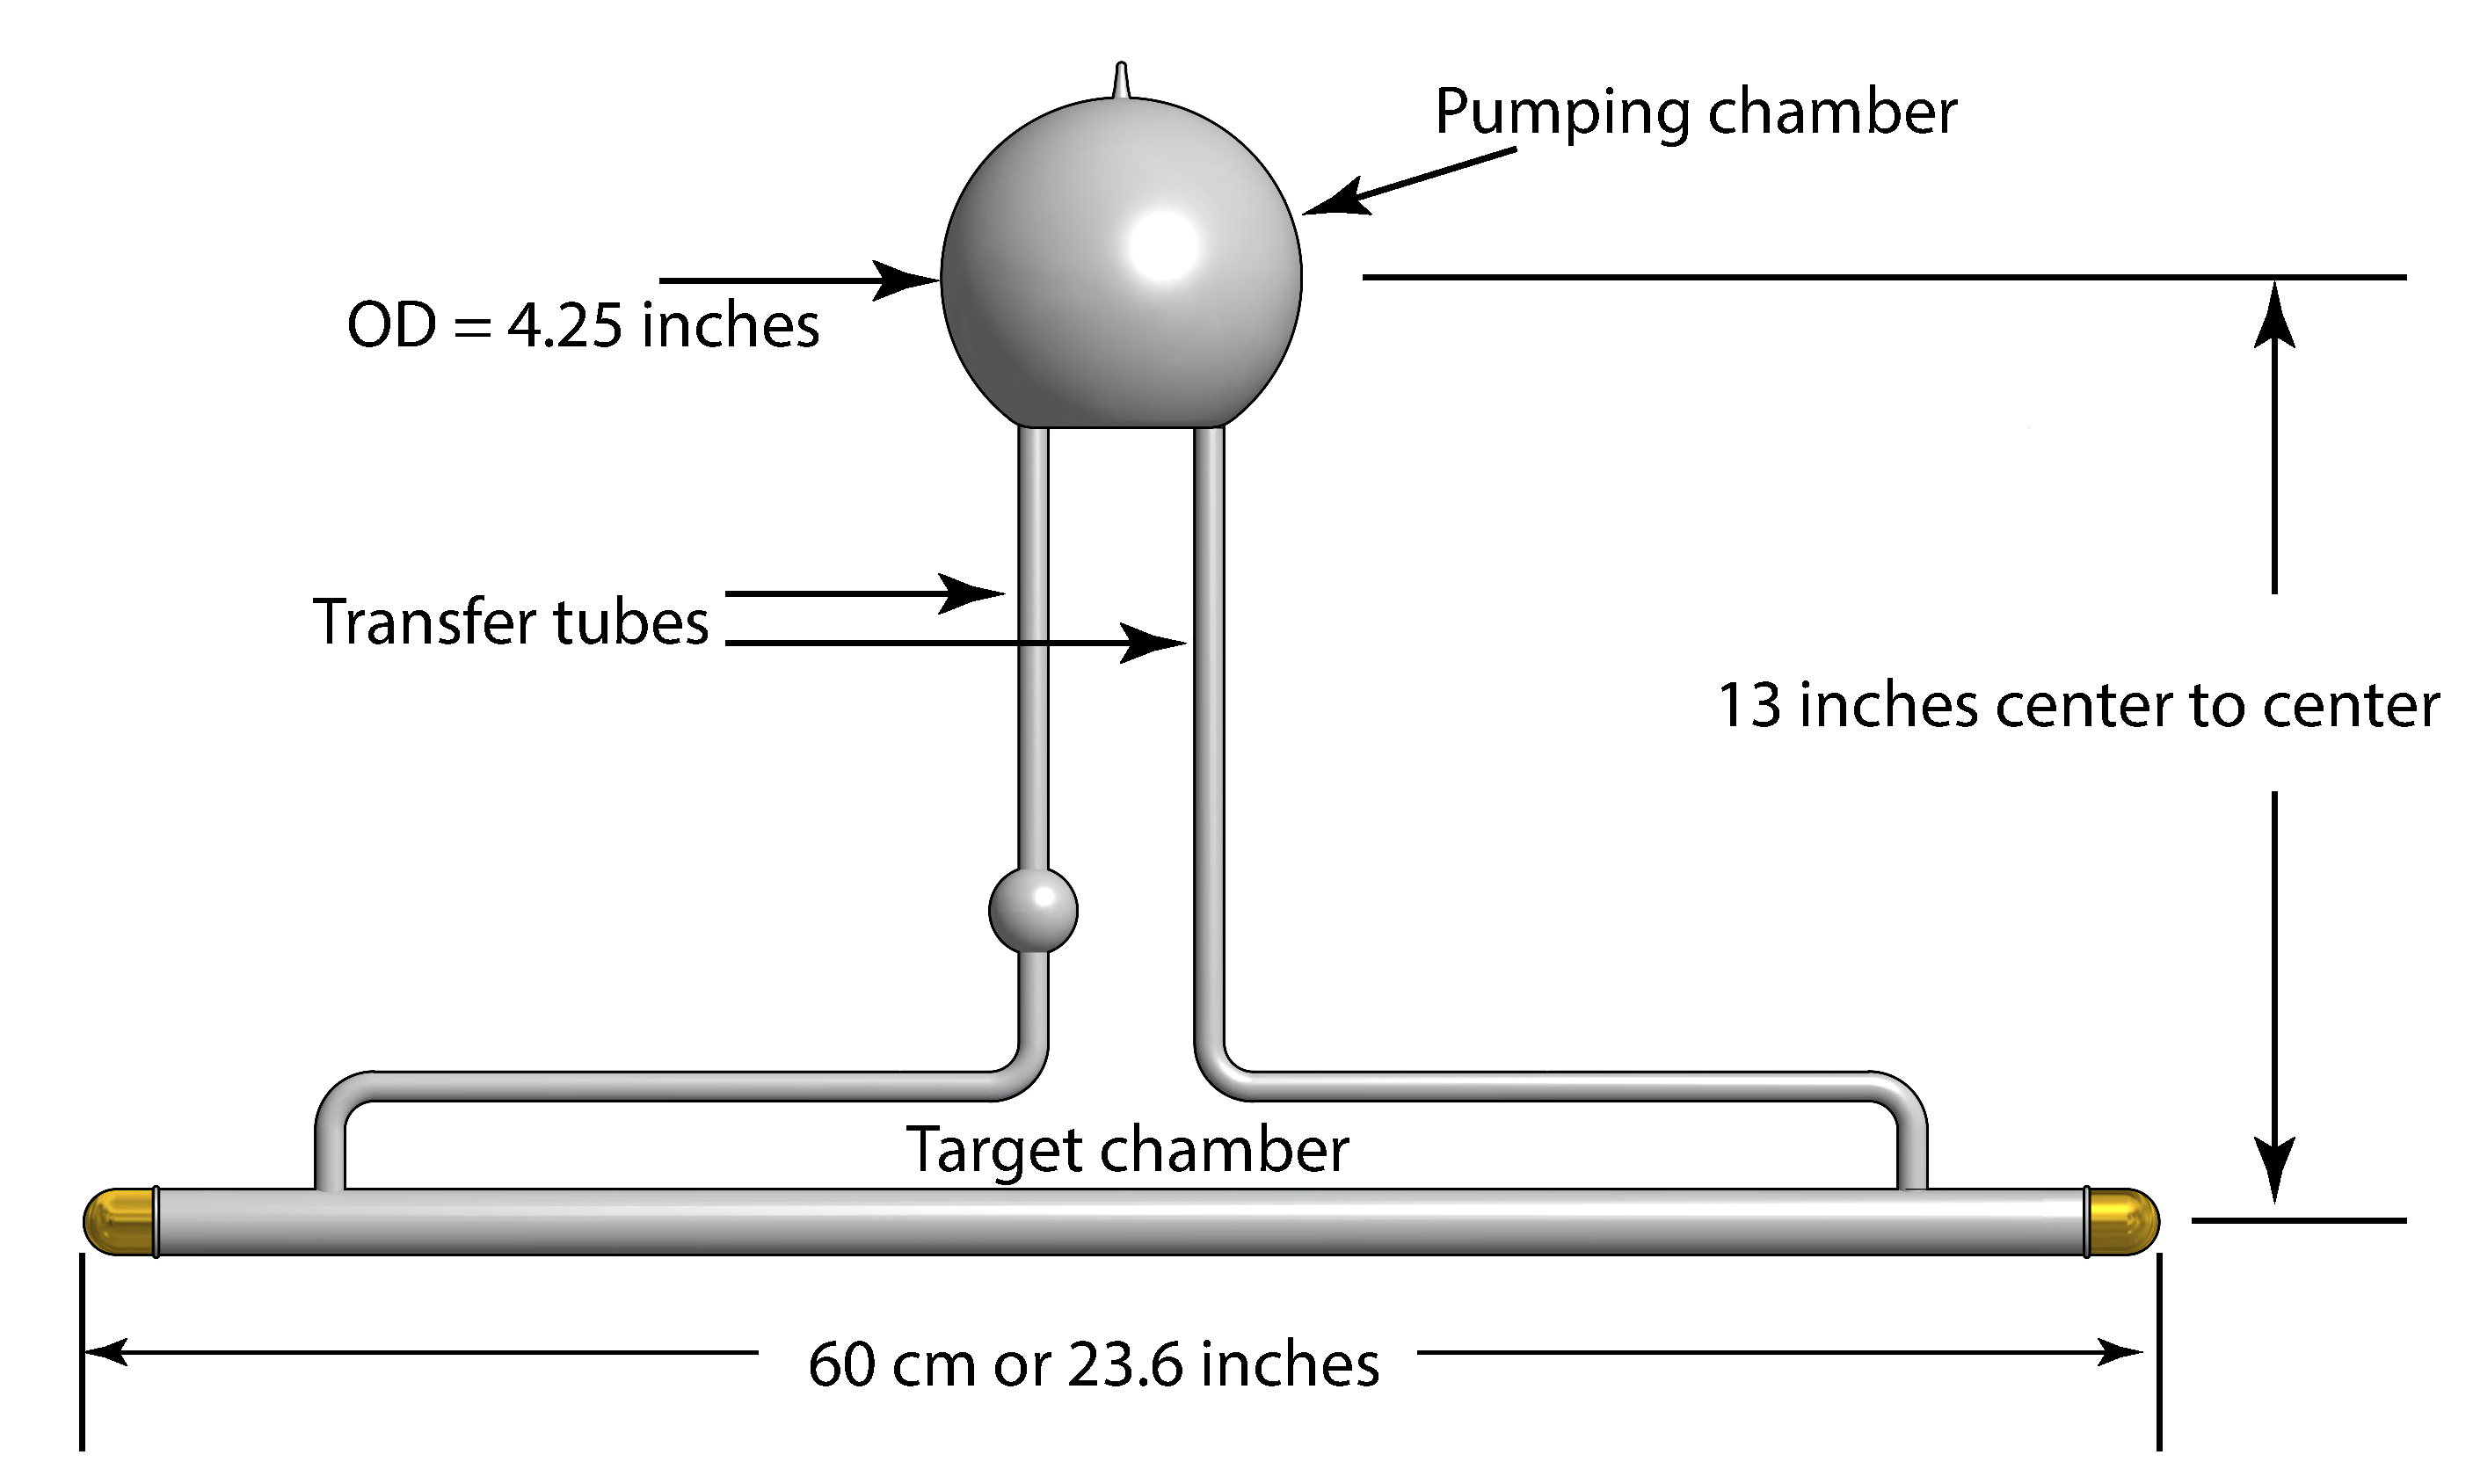
\includegraphics{gen_cell_design_draft_v2.pdf}}
	\caption{{Design of next-generation target for upcoming SBS $G_E^n$ experiments.}}
	\label{Next_Gen_Design}
\end{figure}

\section{Overall Design of Next-Generation Polarized $^3$He Targets}

The target-cell design illustrated in Fig.~\ref{Next_Gen_Design} incorporates multiple features that distinguish it from earlier polarized $^3$He targets based on spin-exchange optical pumping. The basic geometry is what we refer to as a ``convection-style" cell, in which the pumping and target chambers are connected
by two transfer tubes, one of which is heated, resulting in controllable convective flow between the target's two principle chambers. The development of convection-style cells was an important part of the thesis work of Peter Dolph, and is well documented in Ref.~\cite{PhysRevC.84.065201}. Subsequent to the work described in~\cite{PhysRevC.84.065201}, our group constructed and tested two convection-style prototype target cells. 

Another distinguishing feature of the design shown in Fig.~\ref{Next_Gen_Design} is that it is significantly larger than previous target cells, containing 6 STP liters of $^3$He, and has a target chamber that is 60 cm in length, 50\% longer than any target cells previously operated at JLab.  The confidence that this target will achieve polarization $>$ 60\% in ${\rm 60\,\mu A}$ of beam came as a direct result of the work described in Chapter 4, and published in Ref.~\cite{PhysRevC.91.055205}. While much of the data presented in Ref.~\cite{PhysRevC.91.055205} were obtained prior to the work described here, most of the analysis was performed as part of this work, including a determination of the coefficient characterizing spin-exchange between potassium and $^3$He.  

Data included in ref.~\cite{PhysRevC.91.055205} that were specifically obtained as part of this thesis work included all of the studies of the cell Antoinette, which contained roughly 3 STP liters of $^3$He. While target-cells containing 3 STP liters of $^3$He were used during the first Hall A $G_E^n$ experiment (E02-013), commercial narrow-band high-power diode-laser arrays, which are critical to achieving high performance, were not yet available during both testing and the experiment itself. Thus, Antoinette was the first target cell tested with narrow-band lasers that contained both 3 STP liters of $^3$He and an alkali-hybrid mixture for optical pumping. As such, Antoinette became a proof of principle for both of the above-mentioned prototype convection-style target cells, as well as the first production Stage-I target cell that is undergoing testing at the time of this writing.

In short, the work presented here provided the basis for designing the high-performance Stage-I and Stage-II target cells that will be used in future JLab experiments. The proof-of-principle began with the cell Antoinette, and continued with the two prototype convection-style target cells (both of which
also contained roughly 3 STP liters of $^3$He). The first actual Stage-I target cell looks very promising in early tests, providing further confidence in the design of the Stage-II target cells that will soon be produced.

\section{Incorporating Metal End Windows}

Prior to the work described here, there was only very limited experience with spin-polarized noble gases in cells containing metal. The reason is that the introduction of any new material  generally causes spin relaxation greatly in excess to that caused by the walls of the glass container. The target-cell design shown in Fig.~\ref{Next_Gen_Design}, however, incorporates metal end windows so that even a fairly intense electron beam will not cause the target cell to rupture, even after multiple weeks of operation. One of the important achievements
of the current work was the development of a technique for producing metal surfaces that induce spin relaxation at an acceptably slow rate. We further have demonstrated a means for making transitions between glass and metal, even when operating at the high pressures used in our polarized $^3$He targets. We describe
next why metal end windows based on the techniques demonstrated here are likely to have an almost negligible effect on the overall performance of our target cells.

The spin relaxation caused by metal end windows in future target cells can be calculated using the equation $\Gamma_{metal} = \rho_{metal} S_{metal}/V_{total}$ (see Chapter 2.4). Furthermore, the relaxivity associated with metal can be extracted by comparing a glass-and-metal test cell (such as GoldRush in Table.~\ref{test_cells}) with an all-glass control cell (such as Pyrah in Table.\ref{test_cells}). The relaxivity for Pyrah can be computed to be 0.0314 cm/hr, and when compared with GoldRush, indicates a relaxivity of 0.123 cm/hr for the metal. Using this relaxivity and the design dimensions for the target end windows, the additional relaxation times would be 1/93.06 hr$^{-1}$ for Stage-I cells and 1/186.12 hr$^{-1}$ for Stage-II cells.

During the 6 GeV era where only 10-15 $\mu$A was used, glass end windows were already running into risk of rupturing after 4-6 weeks of being exposed to the electron beam. If rupturing was solely due to radiation damage, one would expect the glass windows to rupture after roughly a week of being used in an electron beam of 60 $\mu$A, which would be much less than the time required for the experiment to complete. On the other hand, experience at JLab suggests that even very thin metal windows would be able to survive the electron beam. As a an example, aluminum as thin as 2 mils has been routinely used in JLab without failing. The fact that metal end windows will conduct heat better further suggests that they will be more suitable for the planned experiment. While some work remains to determine the optimal configuration for the window itself, the work presented here provides the critical technology that previously prevented us from using metal end windows in our targets.

\section{Summary}

We have confidence that convection style targets with metal end windows will not only give high $^3$He polarization in both the pumping and target chambers, but also survive the high electron beam currents planned for the future experiments. The work done in this thesis has demonstrated that the additional spin-relaxation rate due to surfaces in metal end windows will be negligible for our purposes and has provided techniques for connecting metal end windows to glass. All the tests so far have been performed on test cells with metal tubes. Before a target cell with next-generation design can be produced, tests exploring techniques for making hemispherical metal end caps should be carried out. However, with techniques established so far, we believe the next-generation design will be used to great success in the upcoming experiments planned for the 12 GeV era.


\include{bib}

% \appendix
% \include{apdxa}
	
\end{document}
